\documentclass[a4paper,14pt]{extarticle}
\usepackage{graphicx}

\usepackage[left=30mm, right=10mm, top=20mm, bottom=20mm]{geometry}
% \usepackage[left=25mm, right=15mm, top=15mm, bottom=15mm]{geometry}
\linespread{1.3} 

\usepackage[T1]{fontenc}
\usepackage[utf8]{inputenc}
\usepackage[english,russian]{babel}

\usepackage{amsmath,amssymb,amsfonts}
\usepackage{amsthm}
\usepackage[colorlinks=true,allcolors=blue]{hyperref}
\usepackage{float}

\usepackage{tocloft}
\renewcommand{\cftsecleader}{\cftdotfill{\cftdotsep}}

\usepackage{caption}
\captionsetup{font=footnotesize}
\captionsetup{labelfont=bf}
\captionsetup{justification=centering}

\pagestyle{myheadings}

% \theoremstyle{definition}
\newtheorem{definition}{Определение}[subsection]
\newcommand{\definitionautorefname}{опр.}
\newtheorem{theorem}{Теорема}[subsection]
\newtheorem{example}{Пример}[subsection]
\newtheorem{lemma}{Лемма}[subsection]
\newcommand{\lemmaautorefname}{лемм.}
\numberwithin{equation}{subsection}

\usepackage{enumitem}

\setlist[enumerate]{leftmargin=*}
\setlist[itemize]{leftmargin=*}

\def\ci{\perp\!\!\!\perp}

% \usepackage{hyperref}
% \hypersetup{pdfstartview={XYZ null null 1.00}}

\bibliographystyle{gost-numeric.bbx}
\RequirePackage[
    parentracker=true,
    backend=biber,
    bibstyle=gost-numeric,
    citestyle=gost-numeric,
    hyperref=true,
    bibencoding=utf8,
    language=auto,
    autolang=other,
    defernumbers=false,
    doi=false,
    eprint=false,
    isbn=false,
    dashed=false,
    url=false
]{biblatex} 
\addbibresource{refs.bib}
\RequirePackage{bibentry}

\begin{document}

% титульник
\thispagestyle{empty}

\begin{center}
    \textsc{
    ФЕДЕРАЛЬНОЕ ГОСУДАРСТВЕННОЕ АВТОНОМНОЕ\\
    ОБРАЗОВАТЕЛЬНОЕ УЧРЕЖДЕНИЕ\\
    ВЫСШЕГО ОБРАЗОВАНИЯ\\
    «НАЦИОНАЛЬНЫЙ ИССЛЕДОВАТЕЛЬСКИЙ УНИВЕРСИТЕТ\\
    «ВЫСШАЯ ШКОЛА ЭКОНОМИКИ»}
\end{center}

\vfill

\begin{center}
    \textbf{Факультет информатики, математики и компьютерных наук}

    \vspace{20pt}

    \textbf{Программа подготовки бакалавров по направлению \\
    01.03.02 Прикладная математика и информатика}
\end{center}

\vfill

\begin{center}
    \textit{Антонов Илья Витальевич} 
    
    \vspace{20pt}
    
    \textbf{ВЫПУСКНАЯ КВАЛИФИКАЦИОННАЯ РАБОТА}

    \vspace{20pt}
    
    Проверка условной независимости в трехмерном распределении Бернулли
\end{center}

\vfill

\begin{flushright}
Научный руководитель

\vspace{5pt}

д.ф.-м.н., проф.

\vspace{5pt}

П.А. Колданов
\end{flushright}

\vfill

\begin{center}
    Нижний Новгород, 2024
\end{center}
\newpage

% содержание
\tableofcontents

\newpage

\section*{Введение}
\addcontentsline{toc}{section}{Введение}

\textbf{Обзор по теме исследования и актуальность} \quad
В современных задачах биоинформатики, информационного поиска,
обработки речи и изображений возникает необходимость изучения
взаимосвязей между большим количеством случайных величин.
Методологию для решения такой проблемы предоставляют графические модели. 
Графической моделью \cite{Jordan2004} называется 
семейство вероятностных распределений, определенное в терминах
ориентированного или неориентированного графа. В этом графе вершины 
соответствуют случайным величинам, 
а ребра отображают некоторые условные зависимости. 
Основным назначением графических моделей является создание
аппарата, упрощающего вычисление
совместных, маргинальных и условных вероятностей.

Наиболее известной графической моделью является 
гауссовская графическая модель \cite{Anderson2003}, в которой рассматриваемые
случайные величины имеют многомерное нормальное распределение. Процедуры
идентификации гауссовской графической модели по наблюдениям
приводятся в работах \cite{Drton2004, Drton2007}. Однако, 
эти процедуры оказываются неустойчивыми к отклонению от многомерного
нормального распределения.
В частности, при таком отклонении тесты проверки индивидуальных гипотез 
не контролируют уровень значимости. 
Кроме того, многомерное нормальное распределение не всегда является
адекватной моделью для описания реальных данных. Поэтому проблема
построения устойчивой графической модели является актуальной. 

Направление построения устойчивой графической модели
для произвольного случайного вектора $(X_1,\ldots,X_N)^T$
целесообразно связать с построением графической модели для
индикаторных случайных величин $(I_1,\ldots,I_N)^T$, где 
$I_i=I(a_i<X_i<b_i)$. 
Возможной графической моделью в таком случае можно назвать
0-1 модель \cite{low_order1}.
В ней ребро между вершинами, которые соответствуют
случайным величинам $I_i$ и $I_j$,
проводится, если выполнены следующие условия:
\begin{itemize}
    \item $I_i$ и $I_j$ маргинально зависимы
    \item $I_i$ и $I_j$ условно зависимы при условии $I_k$
    для всех $k\in \{1,\ldots,N\} \setminus \{i,j\}$
\end{itemize}
Так как совместное распределение индикаторных случайных величинам
описывается многомерным распределением Бернулли 
\cite{Dai2013, Teugels1990}, то
для идентификации 0-1 модели по наблюдениям требуется
теория проверки условной независимости в трехмерном распределении
Бернулли. Построению требуемой теории посвящена
данная работа.
% Естественным обобщением многомерного нормального распределения
% является эллиптическое распределение \cite{Anderson2003}.
% Стоит отметить, что класс многомерных нормальных распределений 
% содержится в классе эллиптических распределений.
% Одним из параметров эллиптического распределения выступает $S$ -- матрица 
% формы (shape matrix), которая при существовании вторых моментов
% компонент эллиптического случайного вектора пропорциональна ковариационной матрице.
% В работе \cite{Vogel2011} для построения эллиптической 
% графической модели, 
% как устойчивого аналога гауссовской графической модели, вводится $K$ -- матрица обобщенных частных корреляций -- как функция от матрицы $S$.
% Ноль в матрице обобщенных частных корреляций
% обозначает условную некоррелированность пары случайных величин при условии
% остальных случайных величин. То есть в отличии от гауссовской
% графической модели, в эллиптической графической модели отсутствие
% ребра обозначает не условную независимость, а условную некоррелированность.
% В работе \cite{Vogel2011} рассматривают 
% $\hat K$ -- оценку матрицы $K$ --
% как функцию от $\hat S$ -- оценки матрицы $S$.
% Для $\hat S$ вводятся некоторые предположения,
% при выполнении которых вектор $Vec(\hat K)$, составленный из элементов $\hat K$, сходится по распределению
% к многомерному нормальному распределению с некоторыми параметрами. 
% Затем приводятся примеры таких оценок $\hat S$, 
% для которых эти предположения выполнены 
% при условии существовании некоторых моментов нормы
% разности эллиптического случайного вектора и его вектора средних.
% Таким образом, наличие оценок для $K$ и их асимптотических распределений приводит к статистической
% теории идентификации эллиптической графической модели.

% Другое направление построения устойчивой графической модели 
% можно связать с переходом от рассмотрения случайных величин $X_i$
% к рассмотрению индикаторных случайных величин $I_i=I(a_i<X_i<b_i)$.
% Условные зависимости между такими случайными величинами естественно
% приводят к графической модели.
% Совместное распределение индикаторных случайных величин описывается
% многомерным распределением Бернулли \cite{Dai2013, Teugels1990}.
% Настоящая выпускная квалификационная работа посвящена проверке условной
% независимости в трехмерном распределении Бернулли. В частности, эта
% теория может быть использована для задачи идентификации графической модели
% с попарным марковским свойством в трехмерном распределении Бернулли.
% Предполагается, что рассмотрение трехмерного случая позволит
% понять перспективность исследований общего многомерного случая.

\textbf{Постановка задачи} \quad
Задачей настоящей выпускной квалификационной работы 
является построение тестов уровня $\alpha$ 
проверки гипотезы \\ $H: X \ci Y \mid Z$
по наблюдениям
$
\begin{pmatrix}
    x_1 \\
    y_1 \\
    z_1
\end{pmatrix},
\begin{pmatrix}
    x_2 \\
    y_2 \\
    z_2
\end{pmatrix}, \ldots,
\begin{pmatrix}
    x_n \\
    y_n \\
    z_n
\end{pmatrix}
$ над случайным вектором $(X,Y,Z)^T$ с
трехмерным распределением Бернулли, а также
анализ свойств этих тестов.


\newpage
\section{Теоретическая часть}

\subsection{Условная независимость в трехмерном распределение Бернулли}\label{ci_and_bernoulli}

Определим трехмерное распределение Бернулли \cite{Dai2013, Teugels1990}.
\begin{definition}
    Случайный вектор $(X,Y,Z)^T$ имеет трехмерное распределение Бернулли,
    если множество его возможных значений:
    $$
        \begin{pmatrix}
            0 \\
            0 \\
            0
        \end{pmatrix},
        \begin{pmatrix}
            0 \\
            0 \\
            1
        \end{pmatrix},
        \begin{pmatrix}
            0 \\
            1 \\
            0
        \end{pmatrix}, \ldots, \begin{pmatrix}
            1 \\
            1 \\
            1
        \end{pmatrix}
    $$ и заданы $P(X=x,Y=y,Z=z)=p_{xyz} \geq 0,  \sum_{x=0}^1 \sum_{y=0}^1 \sum_{z=0}^1 p_{xyz} =1$.
\end{definition}
Приведем определение понятия условной независимости \cite{Lauritzen1996}.
\begin{definition}\label{cond_ind_def}
    Пусть $(X,Y,Z)^T$ -- дискретный случайный вектор.
    Говорят, что случайные величины $X$ и $Y$ условно независимы при условии $Z$,
    и пишут $X \ci Y \mid Z$, если:
    $$
    P(X=x, Y=y \mid Z = z) = P(X=x \mid Z = z) P(Y=y \mid Z = z)
    $$
    при любых $x,y$ и $z$ для которого $P(Z=z)>0$.
\end{definition}
Найдем условия на параметры трехмерного распределения 
Бернулли при условной независимости.
\begin{theorem}\label{thm1}
    Пусть $(X,Y,Z)^T$ -- случайный вектор, имеющий трехмерное распределение Бернулли, в котором $P(Z=0)>0$.
    Случайные величины $X$ и $Y$ условно независимы при условии $Z$ тогда и только тогда, когда
    $$p_{00z}p_{11z}=p_{01z}p_{10z}$$ для всех $z=\overline{0,1}$.
\end{theorem}
\begin{proof}
    Пусть $X \ci Y \mid Z$. Значит, для любых $x=\overline{0,1}$, $y=\overline{0,1}$ и $z=\overline{0,1}$ выполнено условие:
    \begin{equation}\label{ci_cond}
        P(X=x, Y=y \mid Z = z) = P(X=x \mid Z = z) P(Y=y \mid Z = z)
    \end{equation}
    После домножения \eqref{ci_cond} на $P(Z=z)^2>0$ получаем эквивалентное условие:
    \begin{equation}\label{ci_cond2}
        P(X=x,Y=y,Z=z)P(Z=z)=P(X=x,Z=z)P(Y=y,Z=z)
    \end{equation}
    Найдем следующие вероятности:
    $$
        P(X=x, Z=z) = p_{x0z} + p_{x1z},\;  P(Y=y, Z=z) = p_{0yz} + p_{1yz}
    $$
    $$
        P(Z=z)= p_{00z} + p_{01z} + p_{10z} + p_{11z}
    $$
    Тогда условие \eqref{ci_cond2} перепишем в следующем виде:
    $$
        p_{xyz} (p_{00z} + p_{01z} + p_{10z} + p_{11z}) = (p_{x0z} + p_{x1z}) (p_{0yz} + p_{1yz})
    $$
    Это условие выполняется для всех $x=\overline{0,1}$, $y=\overline{0,1}$, $z=\overline{0,1}$.
    Пусть $z$ фиксировано.
    Если $x=0$ и $y=0$, то:
    $$
        p_{00z} (p_{00z} + p_{01z} + p_{10z} + p_{11z}) = (p_{00z} + p_{01z}) (p_{00z} + p_{10z})
    \Leftrightarrow
        p_{00z} p_{11z} = p_{01z} p_{10z}
    $$
    Если $x=0$ и $y=1$, то:
    $$
        p_{01z} (p_{00z} + p_{01z} + p_{10z} + p_{11z}) = (p_{00z} + p_{01z}) (p_{01z} + p_{11z})
    \Leftrightarrow
    p_{00z} p_{11z} = p_{01z} p_{10z}
    $$
    Если $x=1$ и $y=0$, то:
    $$
        p_{10z} (p_{00z} + p_{01z} + p_{10z} + p_{11z}) = (p_{10z} + p_{11z}) (p_{00z} + p_{10z})
    \Leftrightarrow
    p_{00z} p_{11z} = p_{01z} p_{10z}
    $$
    Если $x=1$ и $y=1$, то:
    $$
        p_{11z} (p_{00z} + p_{01z} + p_{10z} + p_{11z}) = (p_{10z} + p_{11z}) (p_{01z} + p_{11z})
    \Leftrightarrow
    p_{00z} p_{11z} = p_{01z} p_{10z}
    $$
    Таким образом, из $X \ci Y \mid Z$ следует
    $p_{00z}p_{11z}=p_{01z}p_{10z}$ для всех $z=\overline{0,1}$.

    Поскольку в вышеприведенных рассуждениях все переходы равносильные,
    мы также доказали, что из из условия $p_{00z}p_{11z}=p_{01z}p_{10z}$ для всех $z=\overline{0,1}$
    следует $X \ci Y \mid Z$.
\end{proof}
Покажем, что существует случайный вектор $(X,Y,Z)^T$ с трехмерным распределением Бернулли, в котором $X \ci Y \mid Z$.
\begin{example}
    Пусть $(X,Y,Z)^T$ имеет трехмерное распределение Бернулли с вероятностями
    $p_{000}=0.15$, $p_{001}=0.1$, $p_{010}=0.3$, $p_{011}=0.1$, $p_{100}=0.05$, $p_{101}=0.1$,
    $p_{110}=0.1$, $p_{111}=0.1$.
    Заметим, что:
    $$p_{000}p_{110}=p_{010}p_{100}=0.015$$ $$p_{001}p_{111}=p_{011}p_{101}=0.01$$
    Следовательно из \autoref{thm1} следует, что $X \ci Y \mid Z$.
\end{example}


\begin{centering}
    \subsection{Частный коэффициент корреляции Пирсона в трехмерном распределении Бернулли}\label{partial_section}
\end{centering}
% Согласно \cite{Anderson2003} в трехмерном нормальном распределении случайные величины 
% $X$ и $Y$ условно независимы при условии $Z$ тогда и только тогда, когда частный коэффициент корреляции Пирсона
% между $X$ и $Y$ принимает нулевое значение.
% Проверим, сохраняется ли это свойство в трехмерном распределении Бернулли.
В данном разделе исследуем свойства частного коэффициента корреляции Пирсона
в трехмерном распределении Бернулли.

Для случайного вектора $(X,Y,Z)^T$ определим ковариационную матрицу:
$$\Sigma =
    \begin{pmatrix}
        \sigma_{XX} & \sigma_{XY} & \sigma_{XZ} \\
        \sigma_{YX} & \sigma_{YY} & \sigma_{YZ} \\
        \sigma_{ZX} & \sigma_{ZY} & \sigma_{ZZ}
    \end{pmatrix}
$$
где $\sigma_{XY}=E[(X-EX)(Y-EY)]$.
Остатками от $X$ и $Y$ при регрессии на $Z$ называются случайные величины:
$$
X^{\prime}=(X-EX)-\dfrac{\sigma_{XZ}}{\sigma_{ZZ}}(Z-EZ)
$$
$$
Y^{\prime}=(Y-EY)-\dfrac{\sigma_{YZ}}{\sigma_{ZZ}}(Z-EZ)
$$
Согласно работе \cite{Cramér1946}, частный коэффициент корреляции Пирсона определяется как коэффициент
корреляции Пирсона между остатками, другими словами:
$$
\rho^{XY \cdot Z}=\dfrac{E(X^{\prime} Y^{\prime})}{\sqrt{E(X^{\prime})^2 E(Y^{\prime})^2}}
$$
Приведем соотношения, которые справедливы
для $\rho^{XY \cdot Z}$ в произвольном распределении.
\begin{lemma}
    Пусть $(X,Y,Z)^T$ -- произвольный случайный вектор. Тогда:
    $$
    \rho^{XY \cdot Z}=\dfrac{\sigma_{XY} \sigma_{ZZ} - \sigma_{XZ} \sigma_{YZ}}{\sqrt{\sigma_{XX}\sigma_{ZZ}-
        \sigma_{XZ}^2}\sqrt{\sigma_{YY}\sigma_{ZZ}-\sigma_{YZ}^2}}=\dfrac{\rho_{XY}-\rho_{XZ}\rho_{YZ}}{\sqrt{1-\rho_{XZ}^2}\sqrt{1-\rho_{YZ}^2}}
    $$
    где $\rho_{XY}, \; \rho_{XZ}, \; \rho_{YZ}$ -- коэффициент корреляции Пирсона
        между случайными величинами $X$ и $Y$, $X$ и $Z$, $Y$ и $Z$
        соответственно.
\end{lemma}
\begin{proof}
    $$E(X^\prime Y^\prime)=E[((X-EX)-\dfrac{\sigma_{XZ}}{\sigma_{ZZ}}(Z-EZ))((Y-EY)-\dfrac{\sigma_{YZ}}{\sigma_{ZZ}}(Z-EZ))]=$$
    $$=\sigma_{XY}-\dfrac{\sigma_{YZ}}{\sigma_{ZZ}}\sigma_{XZ}-\dfrac{\sigma_{XZ}}{\sigma_{ZZ}}\sigma_{YZ}+
    \dfrac{\sigma_{XZ}\sigma_{YZ}}{\sigma_{ZZ}\sigma_{ZZ}}\sigma_{ZZ}=\dfrac{\sigma_{XY}\sigma_{ZZ}-\sigma_{XZ}\sigma_{YZ}}{\sigma_{ZZ}}$$
    Тогда:
    $$
    \rho^{XY \cdot Z}=\dfrac{E(X^{\prime} Y^{\prime})}{\sqrt{E(X^{\prime})^2 E(Y^{\prime})^2}}=\dfrac{\dfrac{\sigma_{XY}\sigma_{ZZ}-\sigma_{XZ}\sigma_{YZ}}{\sigma_{ZZ}}}
    {\sqrt{
        \dfrac{\sigma_{XX}\sigma_{ZZ}-\sigma_{XZ}\sigma_{XZ}}{\sigma_{ZZ}}
    }\sqrt{
        \dfrac{\sigma_{YY}\sigma_{ZZ}-\sigma_{YZ}\sigma_{YZ}}{\sigma_{ZZ}}
    }}=
    $$
    $$
    =\dfrac{\sigma_{XY} \sigma_{ZZ} - \sigma_{XZ} \sigma_{YZ}}{\sqrt{\sigma_{XX}\sigma_{ZZ}-
    \sigma_{XZ}^2}\sqrt{\sigma_{YY}\sigma_{ZZ}-\sigma_{YZ}^2}}=
    $$
    $$
    =\dfrac{\sigma_{ZZ}\sqrt{\sigma_{XX}\sigma_{YY}}
    \left(\dfrac{\sigma_{XY}}{\sqrt{\sigma_{XX}\sigma_{YY}}} 
    - \dfrac{\sigma_{XZ}}{\sqrt{\sigma_{XX}\sigma_{ZZ}}} \dfrac{\sigma_{YZ}}{\sqrt{\sigma_{YY}\sigma_{ZZ}}}\right)}
    {\sqrt{\sigma_{XX}\sigma_{ZZ}-
    \sigma_{XZ}^2}\sqrt{\sigma_{YY}\sigma_{ZZ}-\sigma_{YZ}^2}}=
    $$
    $$
    =\dfrac{\rho_{XY}-\rho_{XZ}\rho_{YZ}}{\sqrt{1-\dfrac{\sigma_{XZ}^2}{\sigma_{XX}\sigma_{ZZ}}}
    \sqrt{1-\dfrac{\sigma_{YZ}^2}{\sigma_{YY}\sigma_{ZZ}}}}
    =\dfrac{\rho_{XY}-\rho_{XZ}\rho_{YZ}}{\sqrt{1-\rho_{XZ}^2}\sqrt{1-\rho_{YZ}^2}}
    $$
\end{proof}

Для дальнейших рассуждений примем следующие обозначения: 
$$p_{x**}=P(X=x), \; p_{*y*}=P(Y=y), \; p_{**z}=P(Z=z)$$ 
$$  p_{xy*}=P(X=x, Y=y),\; p_{x*z}=P(X=x, Z=z), \; p_{*yz}=P(Y=y, Z=z)$$
Найдем значение выражения $\sigma_{XY} \sigma_{ZZ} - \sigma_{XZ} \sigma_{YZ}$ в трехмерном распределении Бернулли.
\begin{lemma}\label{partial_cov}
    Пусть $(X,Y,Z)^T$ -- случайный вектор, имеющий трехмерное распределение Бернулли. Тогда:
    $$\sigma_{XY} \sigma_{ZZ} - \sigma_{XZ} \sigma_{YZ} = p_{**0}(p_{001}p_{111}-p_{011}p_{101}) + p_{**1} (p_{000}p_{110}-p_{010}p_{100})$$
\end{lemma}
\begin{proof}
    Легко проверить, что $\sigma_{ZZ}= p_{**1}(1-p_{**1})$. Найдем соотношение для $\sigma_{XY}$. Воспользуемся формулой $\sigma_{XY}=E(X Y)-E(X)E(Y)$.
    $$E(X Y) = 1 \cdot p_{11*} + 0 \cdot (p_{00*} + p_{01*} + p_{10*})=p_{11*}$$
    Таким образом, $\sigma_{XY}=p_{11*}-p_{1**}p_{*1*}$. Аналогично, $\sigma_{XZ}=p_{1*1}-p_{1**}p_{**1}$ и $\sigma_{YZ}=p_{*11}-p_{*1*}p_{**1}$.
    Преобразуем выражение $\sigma_{XY} \sigma_{ZZ} - \sigma_{XZ} \sigma_{YZ} =$
    $$
        = (p_{11*}-p_{1**}p_{*1*}) p_{**1}(1-p_{**1})
        -(p_{1*1}-p_{1**}p_{**1})(p_{*11}-p_{*1*}p_{**1})=
    $$
    $$
        = p_{11*}p_{**1} - p_{11*}p_{**1}p_{**1} - p_{1**}p_{*1*}p_{**1} 
        -p_{1*1}p_{*11}+p_{1*1}p_{*1*}p_{**1}+p_{1**}p_{**1}p_{*11} =
    $$
    $$
        =(p_{111}p_{**1}+p_{110}p_{**1}) - p_{11*}p_{**1}p_{**1} - p_{1**}p_{*1*}p_{**1} -
    $$ $$
        -p_{1*1}p_{*11}+p_{1*1}p_{*1*}p_{**1}+p_{1**}p_{**1}p_{*11}=
    $$
    \begin{equation}\label{some_step}
        =(p_{111}p_{**1}-p_{1*1}p_{*11})+p_{**1}(p_{110}-p_{11*}p_{**1} - p_{1**}p_{*1*} + p_{1*1}p_{*1*} + p_{1**}p_{*11})
    \end{equation}
    Заметим, что:\\
    1) $
        p_{110}-p_{11*}p_{**1}=p_{110}-p_{110}p_{**1}-p_{111}p_{**1}=
        p_{110}(1-p_{**1})-p_{111}p_{**1}=
    $
    $ 
        =p_{110}p_{**0}-p_{111}p_{**1}
    $\\
    2) $
        -p_{1**}p_{*1*} + p_{1*1}p_{*1*} + p_{1**}p_{*11}=
    $
    $
        -(p_{1*0}+p_{1*1})(p_{*10}+p_{*11})+p_{1*1}(p_{*10}+p_{*11}) + $
        $+(p_{1*0}+p_{1*1})p_{*11}=
        -p_{1*0}p_{*10}+p_{1*1}p_{*11}
    $\\
    Учитывая вышеприведенные соотношения, запишем \eqref{some_step}:
    $$
    (p_{111}p_{**1}-p_{1*1}p_{*11})+p_{**1}((p_{110}p_{**0}-p_{1*0}p_{*10})-(p_{111}p_{**1}-p_{1*1}p_{*11}))=
    $$
    $$
        =(1-p_{**1})(p_{111}p_{**1}-p_{1*1}p_{*11})+p_{**1}(p_{110}p_{**0}-p_{1*0}p_{*10})=
    $$
    \begin{equation}\label{some_step_2}
        =p_{**0}(p_{111}p_{**1}-p_{1*1}p_{*11})+p_{**1}(p_{110}p_{**0}-p_{1*0}p_{*10})
    \end{equation}
    Также заметим, что:\\
    1) $
        p_{111}p_{**1}-p_{1*1}p_{*11} = p_{111}(p_{001}+p_{011}+p_{101}+p_{111})-
        (p_{101}+p_{111})(p_{011}+p_{111})=
    $
    $
        = p_{001}p_{111}-p_{011}p_{101}
    $
    \\
    2) $
        p_{110}p_{**0}-p_{1*0}p_{*10}=
        p_{110}(p_{000}+p_{010}+p_{100}+p_{110})-(p_{100}+p_{110})(p_{010}+p_{110})=
    $
    $
        =p_{000}p_{110}-p_{010}p_{100}
    $\\
    Подставляя преобразованные выражения в \eqref{some_step_2} имеем:
    $$
    \sigma_{XY} \sigma_{ZZ} - \sigma_{XZ} \sigma_{YZ} = p_{**0}(p_{001}p_{111}-p_{011}p_{101}) + p_{**1} (p_{000}p_{110}-p_{010}p_{100})
    $$
\end{proof}
Вышеприведенное соотношение для $\sigma_{XY} \sigma_{ZZ} - \sigma_{XZ} \sigma_{YZ}$ позволяет доказать следующую теорему.
\begin{theorem}\label{1.2}
    Пусть $(X,Y,Z)^T$ -- случайный вектор, имеющий трехмерное распределение Бернулли.
    Если $X \ci Y \mid Z$, то $\rho^{XY \cdot Z}=0$.
\end{theorem}
\begin{proof}
    Пусть $X \ci Y \mid Z$. Тогда по \autoref{thm1}:
    $p_{000}p_{110}=p_{010}p_{100}$ и 
    $p_{001}p_{111}=p_{011}p_{101}$.
    Используя эти соотношения в числителе частного коэффициента корреляции Пирсона и учитывая \autoref{partial_cov}, имеем:
    $$
    \sigma_{XY} \sigma_{ZZ} - \sigma_{XZ} \sigma_{YZ}=p_{**0}(p_{001}p_{111}-p_{011}p_{101}) + p_{**1} (p_{000}p_{110}-p_{010}p_{100})= 0
    $$
    Следовательно, $\rho^{XY \cdot Z}=0$.
\end{proof}
Таким образом, равенство нулю частного коэффициента корреляции Пирсона является необходимым условием условной независимости.
Однако, это условие не является достаточным, так как в обратную сторону \autoref{1.2} неверна. Приведем контрпример.
\begin{example}
    Пусть $p_{000}=0.15$, $p_{001}=0.1$, $p_{010}=0.1$, $p_{011}=0.15$, $p_{100}=0.1$, $p_{101}=0.15$, $p_{110}=0.15$, $p_{111}=0.1$.
    Тогда $p_{**0}=0.5$, $p_{**1}=0.5$ и
    $$\sigma_{XY} \sigma_{ZZ} - \sigma_{XZ} \sigma_{YZ} = p_{**1}(p_{000}p_{110}-p_{010}p_{100}) + p_{**0}(p_{001}p_{111}-p_{011}p_{101})=$$
    $$=0.5 \cdot (0.15 \cdot 0.15 - 0.1 \cdot 0.1) + 0.5 \cdot (0.1 \cdot 0.1 - 0.15 \cdot 0.15) = 0$$
    А значит $\rho^{XY\cdot X}=0$.
    Однако, случайные величины $X$ и $Y$ условно зависимы при условии $Z$ поскольку:
    $$
        p_{000}p_{110}-p_{010}p_{100}=0.15 \cdot 0.15 - 0.1 \cdot 0.1 = 0.0125 \neq 0
    $$
    $$
        p_{001}p_{111}-p_{011}p_{101}=0.1 \cdot 0.1 - 0.15 \cdot 0.15 = -0.0125 \neq 0
    $$
\end{example}

Для оценки частного коэффициента корреляции Пирсона 
можно использовать
выборочный частный коэффициент корреляции Пирсона:
$$r^{XY\cdot Z}=\dfrac{r_{XY}-r_{XZ}r_{YZ}}{\sqrt{1-r_{XY}^2}\sqrt{1-r_{YZ}^2}}$$
где $r_{XY}$, $r_{XZ}$, $r_{YZ}$ -- выборочный коэффициент корреляции Пирсона
между случайными величинами $X$ и $Y$, $X$ и $Z$, $Y$ и $Z$
соответственно.  
Известно \cite{Anderson2003}, что 
в трехмерном нормальном распределении
при истинности гипотезы $H^{\text{Partial}}: \rho^{XY \cdot Z}=0$ статистика
$$
T^{\text{Partial}}=\sqrt{n-3} \dfrac{r^{XY \cdot Z}}{\sqrt{1-(r^{XY \cdot Z})^2}}
$$
имеет распределение Стьюдента с $n-3$ степенями свободы, 
где $n$ -- количество наблюдений.
Тогда тест уровня $\alpha$ проверки гипотезы $H^{\text{Partial}}:\rho^{XY\cdot Z}=0$
против альтернативы $K^{\text{Partial}}:\rho^{XY\cdot Z}\neq 0$
определяется как:
$$
\varphi^{\text{Partial}}(t) = \begin{cases}
    1, \; |t|>C \\ 
    0, \; |t|\leq C
\end{cases}
$$
где константа $C$ удовлетворяет уравнению
$P(T^{\text{Partial}}>C)=1-\alpha/2$.
% Предположим, что $\varphi^{\text{Partial}}$ является тестом
% уровня $\alpha$ для проверки гипотезы $\rho^{XY \cdot Z}=0$ в трехмерном распределении Бернулли. 
% Поскольку из $X \ci Y \mid Z$ следует $\rho^{XY\cdot Z}=0$, то 
% тест $\varphi^{\text{Partial}}$ также является тестом
% уровня $\alpha$ для проверки гипотезы $h: X \ci Y \mid Z$.
В разделе \ref{numerical_exp} с помощью численных экспериментов 
будет проверено контролирует ли тест $\varphi^{\text{Partial}}$
уровень значимости для гипотезы $H^{\text{Partial}}:\rho^{XY\cdot Z}=0$ в трехмерном распределении Бернулли.
% В настоящей работе с помощью численных экспериментов
% будет проверено контролирует ли тест 
% $\varphi^{\text{Partial}}$ вероятность ошибки первого рода
% в трехмерном распределении Бернулли.
% \begin{lemma}
%     Пусть $\Sigma$ -- ковариационная матрица с элементами
%     $$\Sigma =
%     \begin{pmatrix}
%         \sigma_{XX} & \sigma_{XY} & \sigma_{XZ} \\
%         \sigma_{YX} & \sigma_{YY} & \sigma_{YZ} \\
%         \sigma_{ZX} & \sigma_{ZY} & \sigma_{ZZ}
%     \end{pmatrix}
%     $$
%     а $\Sigma^{-1}$ обратная ковариационная матрица с элементами
%     $$\Sigma^{-1} =
%     \begin{pmatrix}
%         \sigma^{XX} & \sigma^{XY} & \sigma^{XZ} \\
%         \sigma^{YX} & \sigma^{YY} & \sigma^{YZ} \\
%         \sigma^{ZX} & \sigma^{ZY} & \sigma^{ZZ}
%     \end{pmatrix}
%     $$
%     Тогда для частного коэффициента корреляции справедливо:
%     $$
%     \rho^{XY \cdot Z}=-\dfrac{\sigma^{XY}}{\sqrt{\sigma^{XX}\sigma^{YY}}}
%     $$
% \end{lemma}
% \begin{proof}
%     Воспользуемся следующими соотношениями для элементов обратной матрицы:
%     $$
%     \sigma^{XY}=\dfrac{-1}{det(\Sigma)}\begin{vmatrix}
%     \sigma_{XY} & \sigma_{XZ}\\
%     \sigma_{YZ} & \sigma_{ZZ}
%     \end{vmatrix}=\dfrac{-(\sigma_{XY}\sigma_{ZZ}-\sigma_{XZ}\sigma_{YZ})}{det(\Sigma)}
%     $$

%     $$
%     \sigma^{XX}=\dfrac{1}{det(\Sigma)}\begin{vmatrix}
%     \sigma_{YY} & \sigma_{YZ}\\
%     \sigma_{YZ} & \sigma_{ZZ}
%     \end{vmatrix}
%     = \dfrac{\sigma_{YY}\sigma_{ZZ}-\sigma_{YZ}^2}{det(\Sigma)}
%     $$

%     $$
%     \sigma^{YY}=\dfrac{1}{det(\Sigma)}\begin{vmatrix}
%     \sigma_{XX} & \sigma_{XZ}\\
%     \sigma_{XZ} & \sigma_{ZZ}
%     \end{vmatrix}
%     = \dfrac{\sigma_{XX}\sigma_{ZZ}-\sigma_{XZ}^2}{det(\Sigma)}
%     $$
%     Тогда:
%     $$
%     -\dfrac{\sigma^{XY}}{\sqrt{\sigma^{XX}\sigma^{YY}}}=-\dfrac{
%         \dfrac{-(\sigma_{XY}\sigma_{ZZ}-\sigma_{XZ}\sigma_{YZ})}{det(\Sigma)}
%     }{
%         \sqrt{\dfrac{\sigma_{XX}\sigma_{ZZ}-\sigma_{XZ}^2}{det(\Sigma)}}
%         \sqrt{\dfrac{\sigma_{YY}\sigma_{ZZ}-\sigma_{YZ}^2}{det(\Sigma)}}
%     }=
%     $$
%     $$
%     = \dfrac{\sigma_{XY}\sigma_{ZZ}-\sigma_{XZ}\sigma_{YZ}}{
%         \sqrt{\sigma_{XX}\sigma_{ZZ}-\sigma_{XZ}^2}
%         \sqrt{\sigma_{YY}\sigma_{ZZ}-\sigma_{YZ}^2}
%     }=\rho^{XY \cdot Z}
%     $$
% \end{proof}

\begin{centering}
    \subsection{Тест на параметр трехмерного распределения Бернулли в экспоненциальной форме}\label{expon_form_section}
\end{centering}
Покажем вид трехмерного распределения Бернулли в экпоненциальной форме:
$$
    P(X=x,Y=y,Z=z) = p_{000}^{(1-x)(1-y)(1-z)} \ldots p_{111}^{x y z} =
$$
$$
    =
        \exp \Biggl\{\ln(p_{000}) +   \ln  \left(\dfrac{p_{001}p_{111}p_{010}p_{100}}{p_{011}p_{101}p_{000}p_{110}}\right)  xyz
     +   \ln\left(\dfrac{p_{100}}{p_{000}}\right) x +   \ln\left(\dfrac{p_{010}}{p_{000}}\right) y + $$
    $$    
    +  \ln\left(\dfrac{p_{001}}{p_{000}}\right) z
        +  \ln \left(\dfrac{p_{000}p_{110}}{p_{010}p_{100}}\right) xy +
         \ln \left(\dfrac{p_{000}p_{101}}{p_{001}p_{100}}\right) xz +
         \ln \left(\dfrac{p_{000}p_{011}}{p_{001}p_{010}}\right) yz \Biggr\}
    $$
Среди параметров, стоящих при статистиках $xyz,x,y,z,xy,xz,yz$ выделим параметр, связанный с условной независимостью.
\begin{theorem}
    Пусть $(X,Y,Z)^T$ -- случайный вектор, имеющий трехмерное распределение Бернулли, и 
    $\theta = \ln  \left(\dfrac{p_{001}p_{111}p_{010}p_{100}}{p_{011}p_{101}p_{000}p_{110}}\right)$.
    Если выполнено одно из условий:
    \begin{itemize}
        \item $X \ci Y \mid Z$
        \item $X \ci Z \mid Y$
        \item $Y \ci Z \mid X$
    \end{itemize}
    то параметр $\theta$ принимает значение $0$.
    \end{theorem}
    
    \begin{proof}
        Результаты теоремы $\ref{thm1}$ можно обобщить следующим образом:
        $$
        X \ci Z \mid Y \Leftrightarrow p_{000}p_{101}=p_{001}p_{100} \text{ и } p_{010}p_{111}=p_{011}p_{110}
        $$
        $$
        Y \ci Z \mid X \Leftrightarrow p_{000}p_{011}=p_{001}p_{010} \text { и } p_{100}p_{111}=p_{101}p_{110}
        $$
        \begin{enumerate}
            \item Пусть $X \ci Y \mid Z$, тогда по теореме \ref{thm1} выполнено:
            $p_{000}p_{110}=p_{010}p_{100}$ и  $p_{001}p_{111}=p_{011}p_{101}$. Отсюда следует, что
            $\theta=\ln(1)=0$.
            \item Пусть $X \ci Z \mid Y$, тогда из вышеприведенных соображений
            $p_{000}p_{101}=p_{001}p_{100}$ и $p_{010}p_{111}=p_{011}p_{110}$. Отсюда следует, что
            $\theta=\ln(1)=0$.
            \item Пусть $Y \ci Z \mid X$, тогда из вышеприведенных соображений
            $p_{000}p_{011}=p_{001}p_{010}$ и $p_{100}p_{111}=p_{101}p_{110}$. Отсюда следует, что
            $\theta=\ln(1)=0$.
        \end{enumerate}
    \end{proof}

    Таким образом, нулевое значение параметра
    $\theta$ является необходимым условием наличия условно независимой пары
    случайных величин в трехмерном распределении Бернулли.
    Для проверки гипотезы о равенстве параметра $\theta$ нулю используем 
    теорию РНМН тестов \cite{Lehmann1986} в многопараметрическом 
    экспоненциальном семействе. Пусть
    $$
        \begin{pmatrix}
            X_1 \\
            Y_1 \\
            Z_1
        \end{pmatrix},
        \begin{pmatrix}
            X_2 \\
            Y_2 \\
            Z_2
        \end{pmatrix}, \ldots,
        \begin{pmatrix}
            X_n \\
            Y_n \\
            Z_n
        \end{pmatrix}
    $$ повторная выборка из распределения случайного вектора $(X,Y,Z)^T$.
    Совместное распределение повторной выборки имеет вид:
    $$
    P(X_1=x_1,Y_1=y_1,Z_1=z_1,\ldots,X_n=x_n,Y_n=y_n,Z_n=z_n)=
    $$
    $$
    =\prod_{i=1}^n P(X_i=x_i,Y_i=y_i,Z_i=z_i) =
    $$
    $$
     =\exp \Biggl\{\ln(p_{000})n + \ln  \left(\dfrac{p_{001}p_{111}p_{010}p_{100}}{p_{011}p_{101}p_{000}p_{110}}\right) \sum_{i=1}^n x_i y_i z_i +$$
        $$ +
            \ln\left(\dfrac{p_{100}}{p_{000}}\right) \sum_{i=1}^{n} x_i + \ln\left(\dfrac{p_{010}}{p_{000}}\right) \sum_{i=1}^{n} y_i +
            \ln\left(\dfrac{p_{001}}{p_{000}}\right) \sum_{i=1}^{n} z_i +
        $$
        $$
            +\ln \left(\dfrac{p_{000}p_{110}}{p_{010}p_{100}}\right) \sum_{i=1}^n x_i y_i +
            \ln \left(\dfrac{p_{000}p_{101}}{p_{001}p_{100}}\right) \sum_{i=1}^n x_i z_i +
            \ln \left(\dfrac{p_{000}p_{011}}{p_{001}p_{010}}\right) \sum_{i=1}^n y_i z_i \Biggr\}
        $$
    Пусть 
    $$
        U = \sum_{i=1}^n X_i Y_i Z_i, \;
        T_1 = \sum_{i=1}^n X_i Y_i, \;
        T_2 = \sum_{i=1}^n X_i Z_i, \;
    $$
    $$
        T_3 = \sum_{i=1}^n Y_i Z_i, \;
        T_4 = \sum_{i=1}^n X_i, \;
        T_5 = \sum_{i=1}^n Y_i, \;
        T_6 = \sum_{i=1}^n Z_i \;
    $$
    Обозначим $T=(T_1,\ldots,T_6)$, $t=(t_1,\ldots,t_6)$, $\theta_0=0$.
    Тогда согласно \cite{Lehmann1986} РНМН тест уровня $\alpha$ проверки гипотезы $\theta=\theta_0$ против альтернативы $\theta \neq \theta_0$ имеет вид:
    $$
    \varphi^{\text{Theta}}(u,t)=\begin{cases}
        1, \; u<C_1(t) \text{ или } u>C_2(t)\\
        \gamma_i, \; u=C_i(t), \; i=1,2\\
        0, \; C_1(t)<u<C_2(t)
    \end{cases}
    $$
    где константы $C_i$ и $\gamma_i$ определяются из системы уравнений:
    $$
    \begin{cases}
        E_{\theta_0}[\varphi^{\text{Theta}}(U,T) \mid T=t]=\alpha \\
        E_{\theta_0}[U\varphi^{\text{Theta}}(U,T) \mid T=t]=\alpha E_{\theta_0}[U \mid T=t]
    \end{cases}
    $$
    Приведем распределение статистики $U$ при условии $T=t$.      
    \begin{lemma}\label{u_dist}
        Пусть $k_1(u)=u$, $k_2(u)=t_1-u$, $k_3(u)=t_2-u$, $k_4(u)=t_3-u$, $k_5(u)=t_4-t_1-t_2+u$, $k_6(u)=t_5-t_1-t_3+u$,
        $k_7(u)=t_6 - t_2 - t_3 + u$, $k_8(u)=n-u+t_1+t_2+t_3-t_4-t_5-t_6$.
        Тогда
        $$P_{\theta_0}(U=u \mid T=t)=\dfrac{(\prod_{i=1}^8 k_i(u)!)^{-1}}
            {\sum_{s\in \mathcal{D}} (\prod_{i=1}^8 k_i(s)!)^{-1}}$$
        где $\mathcal{D}=\{s \in \mathbb{Z}: 0\leq k_i(s) \leq n \text{ для всех } i=1\ldots,8\}$.
    \end{lemma}
    \begin{proof}
        Найдем совместное распределение статистик $(U,T_1,\ldots,T_6)$:
        $$
            P(U=u,T=t)=P(U=u, T_1=t_1, T_2=t_2, T_3=t_3, T_4=t_4, T_5=t_5, T_6=t_6)=
        $$
        $$
            =P\biggl(\sum_{i=1}^n X_i Y_i Z_i=u, \sum_{i=1}^n X_i Y_i=t_1, \sum_{i=1}^n X_i Z_i=t_2,\sum_{i=1}^n Y_i Z_i=t_3,
            $$
            $$
            \sum_{i=1}^n X_i=t_4,\sum_{i=1}^n Y_i=t_5, \sum_{i=1}^n Z_i=t_6\biggr)=
        $$
        $$
            =P\biggl(\sum_{i=1}^n X_i Y_i Z_i=u, \sum_{i=1}^n X_i Y_i (1- Z_i)=t_1-u, \sum_{i=1}^n X_i (1-Y_i) Z_i=t_2-u,
        $$
        $$
            \sum_{i=1}^n (1-X_i) Y_i Z_i=t_3-u,
            \sum_{i=1}^{n} X_i(1-Y_i)(1-Z_i)=t_4-t_1-t_2+u,
        $$
        $$
            \sum_{i=1}^{n} (1-X_i)Y_i(1-Z_i)=t_5-t_1-t_3+u,
            \sum_{i=1}^{n} (1-X_i)(1-Y_i)Z_i = t_6 - t_2 - t_3 + u,
        $$
        $$
            \sum_{i=1}^n (1-X_i)(1-Y_i)(1-Z_i)=n-u+t_1+t_2+t_3-t_4-t_5-t_6\biggr)
            = \frac{n!}{\prod_{i=1}^8 k_i(u)!} \times
        $$
        $$    
        \times p_{111}^u p_{110}^{t_1-u} p_{101}^{t_2-u} p_{011}^{t_3-u}
            p_{100}^{t_4-t_1-t_2+u} p_{010}^{t_5-t_1-t_3+u} p_{001}^{t_6 - t_2 - t_3 + u} 
            p_{000}^{n-u+t_1+t_2+t_3-t_4-t_5-t_6}
            $$
        Тогда условное распределение статистики $U$ при условии $T=t$ можно записать как:
        $$P(U=u \mid T=t)=\dfrac{P(U=u,T=t)}{P(T=t)}=
        \dfrac{P(U=u,T=t)}{\sum_{s \in \mathcal{D}} P(U=s,T=t)}=
        $$
        $$
        =\dfrac{(\prod_{i=1}^8 k_i(u)!)^{-1} \left(\dfrac{p_{001}p_{010}p_{100}p_{111}}{p_{000}p_{011}p_{101}p_{110}}\right)^u}
            {\sum_{s\in \mathcal{D}} (\prod_{i=1}^8 k_i(s)!)^{-1} \left(\dfrac{p_{001}p_{010}p_{100}p_{111}}{p_{000}p_{011}p_{101}p_{110}}\right)^s}$$
        При истинности гипотезы $\theta=\theta_0$ параметр $\dfrac{p_{001}p_{010}p_{100}p_{111}}{p_{000}p_{011}p_{101}p_{110}}=1$. Следовательно:
        $$P_{\theta_0}(U=u \mid T=t)=\dfrac{(\prod_{i=1}^8 k_i(u)!)^{-1}}
            {\sum_{s\in \mathcal{D}} (\prod_{i=1}^8 k_i(s)!)^{-1}}$$
    \end{proof}
    Так как $\varphi^{\text{Theta}}$ является тестом уровня
    $\alpha$ для проверки гипотезы $\theta=\theta_0$, где $\theta_0=0$,
    и из $X \ci Y \mid Z$ следует $\theta=0$, то 
    $\varphi^{\text{Theta}}$ является тестом уровня $\alpha$ для проверки
    гипотезы $h: X \ci Y \mid Z$.
    % Условную вероятность из леммы \ref{u_dist} можно эффективно вычислить на ЭВМ.
    % Пусть $f(i)=\sum_{j=1}^{i} \ln(j)$. Тогда значение условной вероятности представится в виде:
    % $$
    % \dfrac{\frac{1}{\prod_{i=1}^8 k_i(u)!}}{\sum_{s \in D} \frac{1}{\prod_{i=1}^8 k_i(s)!}}=
    % \dfrac{\exp \biggl\{ \ln \biggl( \frac{1}{\prod_{i=1}^8 k_i(u)!} \biggr) \biggr\}}
    % {\sum_{s \in D} \exp \biggl\{ \ln \biggl( \frac{1}{\prod_{i=1}^8 k_i(s)!} \biggr) \biggr\}}
    % = \dfrac{\exp \biggl\{ -\sum_{i=1}^8 \ln(k_i(u)!) \biggr\}}{\sum_{s \in D} \exp \biggl\{ -\sum_{i=1}^8 \ln(k_i(s)!) \biggr\}} =
    % $$
    % $$
    % = \dfrac{\exp \biggl\{ -\sum_{i=1}^8 f(k_i(u)) \biggr\}}{\sum_{s \in D} \exp \biggl\{ -\sum_{i=1}^8 f(k_i(s)) \biggr\}}
    % $$
    % Полученное выражение удобно с позиции того, что современные ЭВМ умеют вычислять функцию
    % $$
    % \varphi(x,i)=\dfrac{\exp\{x_i\}}{\sum_{j=1}^{n} \exp\{x_j\}}, \; x=(x_1,\ldots,x_n)
    % $$
    % За счет свойства
    % $$
    % \varphi(x,i)=\dfrac{\exp\{x_i\}}{\sum_{j=1}^{n} \exp\{x_j\}} = \dfrac{\exp\{x_i - C\}}{\sum_{j=1}^{n} \exp\{x_j - C\}}
    % , \text{ где } C=\max_{1\leq j \leq n} x_j
    % $$
    % удается избежать переполнения вещественного типа данных, связанного с экспонентой.

\begin{center}
    \subsection{РНМН тест проверки независимости в двумерном
распределении Бернулли}\label{bivariate_umpu}
\end{center}
     
В следующем разделе будет показано, что проверку 
условной независимости в трехмерном распределении Бернулли можно 
свести к множественной проверке независимости в условных распределениях.
Согласно работе \cite{Dai2013}, случайный вектор с 
трехмерным распределением Бернулли
при одной фиксированной компоненте имеет
двумерное распределение Бернулли. Приведем теорию проверки независимости
в двумерном распределении Бернулли.

\begin{definition}
    Случайный вектор $(X,Y)^T$ имеет двумерное распределение Бернулли,
    если множество его возможных значений:
    $$
        \begin{pmatrix}
            0 \\
            0
        \end{pmatrix},
        \begin{pmatrix}
            0 \\
            1
        \end{pmatrix},
        \begin{pmatrix}
            1 \\
            0
        \end{pmatrix},
        \begin{pmatrix}
            1 \\
            1
        \end{pmatrix}
    $$ и заданы $P(X=x,Y=y)=p_{xy} \geq 0,  \sum_{x=0}^1 \sum_{y=0}^1 p_{xy} =1$.
\end{definition}

В работе \cite{Dai2013} показано, что:
$$
P(X=x,Y=y)= \exp \left\{\ln(p_{00}) + 
     \ln \left(\dfrac{p_{10}}{p_{00}}\right) x
    +  \ln \left(\dfrac{p_{01}}{p_{00}}\right) y +
     \ln\left(\dfrac{p_{00}p_{11}}{p_{01}p_{10}}\right) xy
 \right\}
$$
Также, в \cite{Dai2013} доказано, что 
$X$ и $Y$ независимы тогда и только тогда, когда
$$\theta=\ln\left(\dfrac{p_{00}p_{11}}{p_{01}p_{10}}\right)=0$$
Пусть
    $$
        \begin{pmatrix}
            X_1 \\
            Y_1 
        \end{pmatrix},
        \begin{pmatrix}
            X_2 \\
            Y_2
        \end{pmatrix}, \ldots,
        \begin{pmatrix}
            X_n \\
            Y_n
        \end{pmatrix}
    $$ повторная выборка из распределения случайного вектора $(X,Y)^T$. Тогда:
$$
    P(X_1=x_1,Y_1=y_1,\ldots,X_n=x_n,Y_n=y_n)
    =\prod_{i=1}^n P(X_i=x_i,Y_i=y_i) =
    $$
    $$
    =\exp \left\{ \ln(p_{00})n + 
        \ln \left(\dfrac{p_{10}}{p_{00}}\right) \sum_{i=1}^n x_i 
        +\ln \left(\dfrac{p_{01}}{p_{00}}\right) \sum_{i=1}^{n} y_i   +
        \ln\left(\dfrac{p_{00}p_{11}}{p_{01}p_{10}}\right) \sum_{i=1}^n x_i y_i 
     \right\}
    $$
    Пусть 
    $$
    U = \sum_{i=1}^n X_i Y_i,\;
    T_1 = \sum_{i=1}^n X_i,\;
    T_2 = \sum_{i=1}^n Y_i
    $$
    Обозначим $T=(T_1,T_2)$, $t=(t_1,t_2)$, $\theta_0=0$.
    Тогда согласно \cite{Lehmann1986} РНМН тест проверки гипотезы $H: \theta = 0$ против альтернативы $K: \theta \neq 0$ 
    уровня $\alpha$ имеет вид:
    $$
    \varphi^{\text{Independence}}(u,t)=\begin{cases}
        1, \; u<C_1(t) \text{ или } u>C_2(t)\\
        \gamma_i, \; u=C_i(t), \; i=1,2\\
        0, \; C_1(t)<u<C_2(t)
    \end{cases}
    $$
    где константы $C_i$ и $\gamma_i$ определяются из системы уравнений:
    $$
    \begin{cases}
        E_{\theta_0}[\varphi^{\text{Independence}}(U,T) \mid T=t]=\alpha \\
        E_{\theta_0}[U\varphi^{\text{Independence}}(U,T) \mid T=t]=\alpha E_{\theta_0}[U \mid T=t]
    \end{cases}
    $$
    Приведем распределение статистики $U$ при условии $T=t$.
\begin{lemma}
    Пусть $k_1(u)=u$, $k_2(u)=t_1-u$, $k_3(u)=t_2-u$,
    $k_4(u)=n-t_1-t_2+u$.
        Тогда
        $$P_{\theta_0}(U=u \mid T=t)=\dfrac{(\prod_{i=1}^4 k_i(u)!)^{-1}}
            {\sum_{s\in \mathcal{D}} (\prod_{i=1}^4 k_i(s)!)^{-1}}$$
        где $\mathcal{D}=\{s \in \mathbb{Z}: 0\leq k_i(s) \leq n \text{ для всех } i=1\ldots,4\}$.
\end{lemma}
Доказательство данной леммы не приводится, поскольку оно полностью 
аналогично доказательству леммы \ref{u_dist}.
% \begin{proof}
%     $$P(U=u,T_1=t_1,T_2=t_2)=
%     P\left(\sum_{i=1}^n X_i Y_i=u,\sum_{i=1}^n X_i=t_1,
%     \sum_{i=1}^n Y_i=t_2\right)=$$
%     $$=P\biggl(
%         \sum_{i=1}^n X_i Y_i=u, \sum_{i=1}^n X_i (1-Y_i)=t_1-u,
%         \sum_{i=1}^n (1-X_i) Y_i=t_2-u,$$
%         $$
%         \sum_{i=1}^n (1-X_i) (1-Y_i)=n-t_1-t_2+u
%         \biggr)
%     =\dfrac{n!}{\prod_{i=1}^{4}k_i(u)!}
%     p_{11}^u p_{10}^{t_1-u} p_{01}^{t_2-u} p_{00}^{n-t_1-t_2+u}
%     $$
%     $$
%     P(U=u \mid T_1=t_1, T_2=t_2)=
%     \dfrac{(\prod_{i=1}^{4}k_i(u)!)^{-1}
%     \left(\dfrac{p_{00}p_{11}}{p_{01}p_{10}}\right)^u}
%     {\sum_{s}(\prod_{i=1}^{4}k_i(s)!)^{-1}
%     \left(\dfrac{p_{00}p_{11}}{p_{01}p_{10}}\right)^s}
%     $$
%     При истинности гипотезы $\theta=0$ параметр 
%     $\dfrac{p_{00}p_{11}}{p_{01}p_{10}}=1$. Тогда:
%     $$
%     P_{\theta=0}(U=u \mid T_1=t_1, T_2=t_2)=
%     \dfrac{(\prod_{i=1}^{4}k_i(u)!)^{-1}}
%     {\sum_{s}(\prod_{i=1}^{4}k_i(s)!)^{-1}}
%     $$
% \end{proof}

\subsection{Процедура проверки условной независимости
в трехмерном распределении Бернулли}\label{twos}

Пусть $(X,Y,Z)^T$ -- случайный вектор, имеющий трехмерное распределение
Бернулли, а
$
\begin{pmatrix}
        x_1 \\
        y_1 \\
        z_1
    \end{pmatrix},
    \begin{pmatrix}
        x_2 \\
        y_2 \\
        z_2
    \end{pmatrix}, \ldots,
    \begin{pmatrix}
        x_n \\
        y_n \\
        z_n
    \end{pmatrix}
$ реализация повторной выборки из распределения $(X,Y,Z)^T$.

Предложим процедуру проверки гипотезы $H: X \ci Y \mid Z$,
контролирующую вероятность ошибки первого рода на уровне $\alpha$:
\begin{itemize}
    \item Разобьем исходную выборку на две подвыборки:
    $$
    \begin{pmatrix}
            x_{i_1} \\
            y_{i_1} \\
            0
        \end{pmatrix},
        \begin{pmatrix}
            x_{i_2} \\
            y_{i_2} \\
            0
        \end{pmatrix}, \ldots,
        \begin{pmatrix}
            x_{i_{n_0}} \\
            y_{i_{n_0}} \\
            0
        \end{pmatrix}
    \text{ и }
    \begin{pmatrix}
            x_{j_1} \\
            y_{j_1} \\
            1
        \end{pmatrix},
        \begin{pmatrix}
            x_{j_2} \\
            y_{j_2} \\
            1
        \end{pmatrix}, \ldots,
        \begin{pmatrix}
            x_{j_{n_1}} \\
            y_{j_{n_1}} \\
            1
        \end{pmatrix}
    $$
    \item По наблюдениям 
    $
    \begin{pmatrix}
        x_{i_1} \\
        y_{i_1} 
    \end{pmatrix},
    \begin{pmatrix}
        x_{i_2} \\
        y_{i_2}
    \end{pmatrix}, \ldots,
    \begin{pmatrix}
        x_{i_{n_0}} \\
        y_{i_{n_0}}
    \end{pmatrix}
    $, которые являются реализацией повторной выборки
    из распределения $(X,Y)^T$ при условии $Z~=~0$,
тестом $\varphi^{\text{Independence}}$ (из \autoref{bivariate_umpu}) уровня $\gamma$
проверим гипотезу $H_0 : X$ и $Y$ независимы при условии $Z=0$. 
Если подвыборка не содержит наблюдений, то применяем тест 
$\varphi \equiv \gamma$.
\item По наблюдениям 
    $
    \begin{pmatrix}
        x_{j_1} \\
        y_{j_1} 
    \end{pmatrix},
    \begin{pmatrix}
        x_{j_2} \\
        y_{j_2}
    \end{pmatrix}, \ldots,
    \begin{pmatrix}
        x_{j_{n_1}} \\
        y_{j_{n_1}}
    \end{pmatrix}
    $, которые являются реализацией 
    повторной выборки из распределения 
    $(X,Y)^T$ при условии $Z~=~1$,
тестом $\varphi^{\text{Independence}}$ (из \autoref{bivariate_umpu}) уровня $\gamma$
проверим гипотезу $H_1 : X$ и $Y$ независимы при условии $Z=1$.
Если подвыборка не содержит наблюдений, то применяем тест 
$\varphi \equiv \gamma$.
\item 
Для проверки гипотезы $H: X \ci Y \mid Z$ используем тест
объединения-пересечения \cite{Roy1953}:
$$
\varphi^{\text{Subsamples}}=\begin{cases}
    1, \text{ наступило событие $A_0 \cup A_1$}\\
    0, \text{ иначе}
\end{cases}
$$
где $A_0 = \{\text{гипотеза $H_0$ отвергнута}\},\;
A_1 = \{\text{гипотеза $H_1$ отвергнута}\}$.
\end{itemize}
\begin{remark}
    Очевидно, что
события $A_0$ и $A_1$ независимые. Поэтому для контроля
$\Prb_{H}(\varphi^{\text{Subsamples}}=1)=\alpha$ достаточно положить
$\gamma = 1 - \sqrt{1-\alpha}$.
\end{remark}
\begin{remark}
    Использование в вышеприведенной процедуре теста\\
    $\varphi^{\text{Independence}}$ объясняется тем, что
    случайный вектор $(X,Y)^T$ при условии $Z~=~z$ имеет двумерное
    распределение Бернулли \cite{Dai2013}.
\end{remark}

% \newpage
% \subsection{Проверка условной независимости по подвыборкам из условных распределений}\label{twos}

% Приведем трактовку \autoref{cond_ind_def} для трехмерного
% распределения Бернулли. 
% \begin{definition}\label{new_def}
%     В трехмерном распределении Бернулли случайные величины $X$ и $Y$
%     условно независимы при условии $Z$, 
%     если выполнены следующие условия:
%     \begin{itemize}
%         \item $X$ и $Y$ независимы при условии $Z=0$
%         \item $X$ и $Y$  независимы при условии $Z=1$
%     \end{itemize}
% \end{definition}
% Используя \autoref{new_def}, сформулируем индивидуальные гипотезы:
% \begin{itemize}
%     \item $H_0 : X$ и $Y$ независимы при условии $Z=0$
%     \item $H_1 : X$ и $Y$ независимы при условии $Z=1$
% \end{itemize}
% Тогда гипотеза об условной независимости имеет вид 
% $H = H_0 \cap H_1$. Естественным образом, гипотезу 
% $H_0$ необходимо проверять по наблюдениям
% $(x_i,y_i,z_i)^T$, в которых $z_i=0$. Поскольку $(X,Y)^T$ при условии
% $Z=z$ имеет двумерное распределение Бернулли, то
% в качестве теста для $H_0$ можно использовать
% $\varphi_0 = \varphi^{\text{Independence}}_0$, 
% приведенный в \autoref{bivariate_umpu}. Аналогичные рассуждения 
% справедливы и для гипотезы $H_1$. Учитывая озвученные соображения,
% построим тест проверки гипотезы $H$, контролирующий вероятность
% ошибки первого рода на уровне $\alpha$.
% Пусть
% $$
% \begin{pmatrix}
%         X_1 \\
%         Y_1 \\
%         Z_1
%     \end{pmatrix},
%     \begin{pmatrix}
%         X_2 \\
%         Y_2 \\
%         Z_2
%     \end{pmatrix}, \ldots,
%     \begin{pmatrix}
%         X_n \\
%         Y_n \\
%         Z_n
%     \end{pmatrix}
% $$ повторная выборка из распределения случайного вектора $(X,Y,Z)^T$. Обозначим $\mathbf{Z}=(Z_1,\ldots,Z_n)$ и 
% $\mathbf{z}=(z_1,\ldots,z_n)$.
% Покажем, что в условном распределении при $\mathbf{Z}=\mathbf{z}$ наблюдения
% $$
% \Xi = 
% \begin{pmatrix}
%         X_1 \\
%         Y_1
%     \end{pmatrix},
%     \begin{pmatrix}
%         X_2 \\
%         Y_2
%     \end{pmatrix}, \ldots,
%     \begin{pmatrix}
%         X_n \\
%         Y_n
%     \end{pmatrix}
% $$
% являются независимыми. 

% \begin{lemma}\label{ci_for_samples}
%     $$
%     P(X_1=x_1,Y_1=y_1,\ldots,X_n=x_n,Y_n=y_n \mid \mathbf{Z}=\mathbf{z})=
%     $$
%     $$
%     =\prod_{i=1}^n P(X_i=x_i, Y_i=y_i \mid \mathbf{Z}=\mathbf{z})
%     $$
% \end{lemma}
% \begin{proof}
%     С одной стороны:
%     $$
%     P(X_1=x_1,Y_1=y_1,Z_1=z_1,\ldots,X_n=x_n,Y_n=y_n,Z_n=z_n)=
%     $$
%     $$
%     =P(\mathbf{Z}=\mathbf{z}) P(X_1=x_1,Y_1=y_1,\ldots,X_n=x_n,Y_n=y_n \mid \mathbf{Z}=\mathbf{z}) 
%     $$
%     С другой стороны:
%     $$
%     P(X_1=x_1,Y_1=y_1,Z_1=z_1,\ldots,X_n=x_n,Y_n=y_n,Z_n=z_n)=
%     $$
%     $$
%     =\prod_{i=1}^n P(X_i=x_i, Y_i=y_i, Z_i=z_i)=
%     $$
%     $$
%     =\prod_{i=1}^n P(X_i=x_i, Y_i=y_i \mid Z_i=z_i)P(Z_i=z_i)=
%     $$
%     $$
%     =P(\mathbf{Z}=\mathbf{z})\prod_{i=1}^n P(X_i=x_i, Y_i=y_i \mid \mathbf{Z}=\mathbf{z})
%     $$
% \end{proof}

% Пусть также $\mathbf{Z}=\mathbf{z}$ фиксированы. 
% Разобьем выборку $\Xi$ на две подвыборки $\Xi_0$ и $\Xi_1$, 
% такие что:
% $$
% \Xi_0=
% \begin{pmatrix}
%     X_{i_1} \\
%     Y_{i_1} \\
% \end{pmatrix},
% \begin{pmatrix}
%     X_{i_2} \\
%     Y_{i_2} \\
% \end{pmatrix}, \ldots,
% \begin{pmatrix}
%     X_{i_{n_0}} \\
%     Y_{i_{n_0}} \\
% \end{pmatrix} 
% $$
% где $Z_{i_k}=z_{i_k}=0$ для всех $i_k$ при $k=\overline{1,n_0}$ и $$
% \Xi_1=
% \begin{pmatrix}
%     X_{j_1} \\
%     Y_{j_1} \\
% \end{pmatrix},
% \begin{pmatrix}
%     X_{j_2} \\
%     Y_{j_2} \\
% \end{pmatrix}, \ldots,
% \begin{pmatrix}
%     X_{j_{n_1}} \\
%     Y_{j_{n_1}} \\
% \end{pmatrix} 
% $$
% где $Z_{j_k}=z_{j_k}=1$ для всех $j_k$ при $k=\overline{1,n_1}$. 
% Причем $n=n_0+n_1$. Отметим, что
% разбиение $\Xi = \Xi_0 \sqcup \Xi_1$ определяется лишь набором
% $\mathbf{Z}=\mathbf{z}$.

% Сформулируем следующую теорему.

% \begin{theorem}
%     Пусть $\mathbf{Z}=\mathbf{z}$ -- фиксированы. Тогда выборка $\Xi_0$ является повторной выборкой из распределения $(X,Y)^T$ при условии $Z=0$.
% \end{theorem}
% \begin{proof}
%     По \autoref{ci_for_samples}:
%     $$
%     P(X_1=x_1,Y_1=y_1,\ldots,X_n=x_n,Y_n=y_n \mid \mathbf{Z}=\mathbf{z})=
%     $$
%     $$
%     =\prod_{i=1}^n P(X_i=x_i, Y_i=y_i \mid \mathbf{Z}=\mathbf{z})
%     $$
%     Просуммировав обе части вышепредставленного равенства по всем возможным значениям 
%     $x_{j_1}, y_{j_1}, \ldots, x_{j_{n_1}},y_{j_{n_1}}$ получаем:
%     $$
%     P(X_{i_1}=x_{i_1},Y_{i_1}=y_{i_1},\ldots,X_{i_{n_0}}=x_{i_{n_0}},Y_{i_{n_0}}=y_{i_{n_0}} \mid \mathbf{Z}=\mathbf{z})=
%     $$
%     $$
%     =\prod_{k=1}^{n_0} P(X_{i_k}=x_{i_k}, Y_{i_k}=y_{i_k} \mid \mathbf{Z}=\mathbf{z})
%     $$
%     Значит $$
%     \Xi_0=
%     \begin{pmatrix}
%         X_{i_1} \\
%         Y_{i_1} \\
%     \end{pmatrix},
%     \begin{pmatrix}
%         X_{i_2} \\
%         Y_{i_2} \\
%     \end{pmatrix}, \ldots,
%     \begin{pmatrix}
%         X_{i_{n_0}} \\
%         Y_{i_{n_0}} \\
%     \end{pmatrix} 
%     $$
%     независимые наблюдения при условии $\mathbf{Z}=\mathbf{z}$.

%     Покажем, что $(X_{i_k},Y_{i_k})^T$ при условии $\mathbf{Z}=\mathbf{z}$ распределен также как и 
%     $(X,Y)^T$ при условии $Z=0$.
%     $$
%     P(X_{i_k}=x_{i_k}, Y_{i_k}=y_{i_k} \mid \mathbf{Z}=\mathbf{z}) =
%     P(X_{i_k}=x_{i_k}, Y_{i_k}=y_{i_k} \mid Z_{i_k}=z_{i_k}) = $$
%     $$=P(X_{i_k}=x_{i_k}, Y_{i_k}=y_{i_k} \mid Z_{i_{k}}=0)=
%     P(X=x_{i_k}, Y=y_{i_k} \mid Z=0)$$
% \end{proof}

% Аналогично показывается, что $\Xi_1$ является повторной выборкой из распределения $(X,Y)^T$ при условии $Z=1$.

% Сформулируем теорему.
% \begin{theorem}\label{main_theorem}
%     Пусть $\Xi_0$ и $\Xi_1$ -- подвыборки, полученные разбиением случайной выборки $\Xi$.
%     Пусть $\varphi_0$ и $\varphi_1$ -- рандомизированные тесты 
%     проверки гипотез $H_0$ и $H_1$ по повторным выборкам 
%     $\Xi_0$ и $\Xi_1$ соответственно.
%     Введем события:
%     $$A_0 = \{\text{отвергнуть гипотезу $H_0$ рандомизированным тестом $\varphi_0$}\}$$ 
%     $$A_1 = \{\text{отвергнуть гипотезу $H_1$ рандомизированным тестом $\varphi_1$}\}$$
%     Пусть $\varphi_0$ и $\varphi_1$ тесты уровня $\alpha_0$ и $\alpha_1$
%     при любом объеме наблюдений в подвыборках $\Xi_0$ и $\Xi_1$ соответственно, то есть:
%     $$P_{H_0\cap H_1,\mathbf{Z=z}}(A_0)=\alpha_0$$ 
%     $$P_{H_0\cap H_1,\mathbf{Z=z}}(A_1)=\alpha_1$$
%     Тогда $P_{H_0\cap H_1}(A_0 \cap A_1)= P_{H_0\cap H_1}(A_0) P_{H_0\cap H_1}(A_1)$.
% \end{theorem}
% \begin{proof}
%     Пусть $\mathbf{Z}=\mathbf{z}$ фиксировано. 
%     Обозначим через
%     $$T_0=(X_{i_1},Y_{i_1},\ldots,X_{i_{n_0}},Y_{i_{n_0}})^T, \;
%     T_1=(X_{j_1},Y_{j_1},\ldots,X_{j_{n_1}},Y_{j_{n_1}})^T$$
%     случайные векторы наблюдений, используемые в тестах $\varphi_0$ и 
%     $\varphi_1$ соответственно.
%     Распишем следующую вероятность
%     $$
%     P_{H_0\cap H_1,\mathbf{Z=z}}(A_0 \cap A_1)=
%     $$
%     $$
%     =\sum_{t_0}\sum_{t_1} P_{H_0\cap H_1,\mathbf{Z=z}}(A_0 \cap A_1 \mid T_0=t_0, T_1=t_1)P_{H_0\cap H_1,\mathbf{Z=z}}(T_0=t_0, T_1=t_1)
%     $$
%     Отметим, что $P_{H_0\cap H_1,\mathbf{Z=z}}(A_0 \cap A_1 \mid T_0=t_0, T_1=t_1)=\varphi_0(t_0)\varphi_1(t_1)$, поскольку
%     для того, чтобы при известных значениях статистик $t_0$ и $t_1$ отвергнуть гипотезы $H_0$ и $H_1$, в рандомизированном тесте нужно провести два испытания с вероятностью успеха
%     $\varphi_0(t_0)$ и $\varphi_1(t_1)$. Постулируется, что такие испытания независимые. Тогда:
%     $$
%     P_{H_0\cap H_1,\mathbf{Z=z}}(A_0 \cap A_1)=\sum_{t_0}\sum_{t_1} \varphi_0(t_0) \varphi_1(t_1) P_{H_0\cap H_1,\mathbf{Z=z}}(T_0=t_0, T_1=t_1)=
%     $$
%     $$
%     =\sum_{t_0}\sum_{t_1} \varphi_0(t_0) \varphi_1(t_1) P_{H_0\cap H_1,\mathbf{Z=z}}(T_0=t_0)P_{H_0\cap H_1,\mathbf{Z=z}}(T_1=t_1)=
%     $$
%     $$
%     =\sum_{t_0}\left[ \varphi_0(t_0) P_{H_0\cap H_1,\mathbf{Z=z}}(T_0=t_0) \left(\sum_{t_1}\varphi_1(t_1) P_{H_0\cap H_1,\mathbf{Z=z}}(T_1=t_1)\right)\right]=
%     $$
%     $$
%     = \sum_{t_0} \varphi_0(t_0) P_{H_0\cap H_1,\mathbf{Z=z}}(T_0=t_0) \alpha_1 
%     =\alpha_0 \alpha_1
%     $$
%     По формуле полной вероятности:
%     $$
%     P_{H_0\cap H_1}(A_0) = \sum_{\mathbf{z}} P_{H_0\cap H_1,\mathbf{Z=z}}(A_0) P_{H_0\cap H_1}(\mathbf{Z}=\mathbf{z})
%     = \sum_{\mathbf{z}} \alpha_0 P_{H_0\cap H_1}(\mathbf{Z}=\mathbf{z})=\alpha_0
%     $$
%     Аналогично, $P_{H_0\cap H_1}(A_1)=\alpha_1$. Также по формуле полной вероятности:
%     $$
%     P_{H_0\cap H_1}(A_0 \cap A_1) = \sum_{\mathbf{z}} P_{H_0\cap H_1,\mathbf{Z=z}}(A_0 \cap A_1) P_{H_0\cap H_1}(\mathbf{Z}=\mathbf{z})=
%     $$
%     $$
%     = \sum_{\mathbf{z}} \alpha_0 \alpha_1 P_{H_0\cap H_1}(\mathbf{Z}=\mathbf{z})
%     = \alpha_0 \alpha_1
%     $$
%     Таким образом, $P_{H_0\cap H_1}(A_0 \cap A_1)=P_{H_0\cap H_1}(A_0) P_{H_0\cap H_1}(A_1)=\alpha_0 \alpha_1$.
% \end{proof}
% Применим \autoref{main_theorem} для проверки условной независимости в трехмерном
% распределении Бернулли.
% Положим индивидуальные гипотезы:
% \begin{itemize}
%     \item $H_0 : X$ и $Y$ независимы при условии $Z=0$
%     \item $H_1 : X$ и $Y$ независимы при условии $Z=1$
% \end{itemize}
% Для проверки гипотез $H_0$ и $H_1$ будем использовать тесты
% $\varphi_0 = \varphi^{\text{Independence}}_0$ и 
% $\varphi_1 = \varphi^{\text{Independence}}_1$ уровня $\alpha_0$ и $\alpha_1$ 
% по повторным выборкам
% $\Xi_0$ и $\Xi_1$ соответственно.
% Тогда гипотеза
% об условной независимости имеет вид $H = H_0 \cap H_1$ и тест проверки условной независимости можно определить как:
% $$
% \varphi^{\text{Subsamples}}=\begin{cases}
%     1, \text{ наступило событие $A_0 \cup A_1$}\\
%     0, \text{ иначе}
% \end{cases}
% $$
% Пусть далее $\alpha_0 = \alpha_1 = \gamma$.
% Тогда $$P_{H_0\cap H_1}(\varphi^{\text{Subsamples}}=1)=P_{H_0\cap H_1}(A_0 \cup A_1)=$$ 
% $$ = P_{H_0\cap H_1}(A_0) + P_{H_0\cap H_1}(A_1) - 
% P_{H_0\cap H_1}(A_0 \cap A_1) = 2\gamma - \gamma^2$$
% Нетрудно проверить, что для контроля $P_{H_0\cap H_1}(\varphi^{\text{Subsamples}}=1)=\alpha$ достаточно положить
% уровень значимости $\gamma = 1 - \sqrt{1-\alpha}$ на
% тестах проверки индивидуальных гипотез $H_0$ и $H_1$.

% Покажем, что тест $\varphi^{\text{Subsamples}}$ является несмещенным.
% \begin{theorem}\label{unbias}
%     Тест $\varphi^{\text{Subsamples}}$
%     уровня $\alpha$
%     проверки гипотезы 
%     $H: X \ci Y \mid Z$ является несмещенным.
% \end{theorem}
% \begin{proof}
%     Положим $\Theta_{H}=\{\theta: p_{000}p_{110}=p_{010}p_{100}
%     \text{ и } p_{001}p_{111}=p_{011}p_{101}\}$, 
%     $\Theta_{K}=\{\theta: p_{000}p_{110}\neq p_{010}p_{100}
%     \text{ или } p_{001}p_{111}\neq p_{011}p_{101}\}$.

%     Отметим, что $\varphi_0 = \varphi^{\text{Independence}}_0$ и
%     $\varphi_1 = \varphi^{\text{Independence}}_1$ -- несмещенные тесты
%     проверки гипотез  $H_0$ и $H_1$ уровня $\gamma$
%     соответственно. Причем, при истинности гипотез $H_0$
%     и $H_1$ на тестах $\varphi_0$ и $\varphi_1$ вероятность ошибки
%     первого рода в точности равна $\gamma$.
%     Поэтому,
%     $E_{\theta}(\varphi_0) = P_\theta(A_0)\geq \gamma$ и $E_{\theta}(\varphi_1) = P_\theta(A_1)\geq \gamma$ для любого
%     $\theta \in \Theta_{H} \cup \Theta_{K}$.

%     Пусть $\theta \in \Theta_{H}$, тогда
%     $E_{\theta}(\varphi^{\text{Subsamples}}) =
%     P_{\theta}(\varphi^{\text{Subsamples}}=1) = \alpha$ поскольку
%     $\varphi^{\text{Subsamples}}$ тест уровня $\alpha$.

%     Пусть $\theta \in \Theta_{K}$.
%     Как и в доказательстве \autoref{main_theorem} можно показать, что
%     $P_{\theta,\mathbf{Z}=\mathbf{z}}(A_0 \cap A_1)=
%     P_{\theta,\mathbf{Z}=\mathbf{z}}(A_0)
%     P_{\theta,\mathbf{Z}=\mathbf{z}}(A_1)$.
%     Следовательно: 
%     $$P_{\theta,\mathbf{Z}=\mathbf{z}}(A_0 \cup A_1) 
%     = P_{\theta,\mathbf{Z}=\mathbf{z}}(A_0) +
%     P_{\theta,\mathbf{Z}=\mathbf{z}}(A_1) - 
%     P_{\theta,\mathbf{Z}=\mathbf{z}}(A_0)
%     P_{\theta,\mathbf{Z}=\mathbf{z}}(A_1) 
%     \geq \gamma + \gamma - \gamma^2 = \alpha
%     $$
%     Тогда:
%     $$
%     E_{\theta}(\varphi^{\text{Subsamples}}) =
%     P_{\theta}(\varphi^{\text{Subsamples}}=1)=
%     P_{\theta}(A_0 \cup A_1)=
%     $$
%     $$
%     =\sum_{\mathbf{z}} P_{\theta,\mathbf{Z}=\mathbf{z}}(A_0 \cup A_1)P_{\theta}(\mathbf{Z}=\mathbf{z}) \geq
%     \sum_{\mathbf{z}} \alpha P_{\theta}(\mathbf{Z}=\mathbf{z}) = \alpha
%     $$
    
% \end{proof}



% \section{Тест проверки условной независимости в трехмерном нормальном распределении}
Пусть
$$
\begin{pmatrix}
    X_1\\
    Y_1 \\
    Z_1
\end{pmatrix}, \begin{pmatrix}
    X_2\\
    Y_2 \\
    Z_2
\end{pmatrix}, \ldots, 
\begin{pmatrix}
    X_n \\
    Y_n \\
    Z_n
\end{pmatrix}
$$
повторная выборка из распределения $(X,Y,Z)^T$ с трехмерным нормальным распределением $\mathcal{N}(\mu, \Sigma)$,
где $\mu$ -- вектор математических ожиданий, а $\Sigma$ -- ковариационная матрица:
$$
\mu = \begin{pmatrix}
    EX \\ EY \\ EZ
\end{pmatrix}, 
\;
\Sigma = \begin{pmatrix}
    \sigma_{XX} & \sigma_{XY} & \sigma_{XZ} \\
    \sigma_{YX} & \sigma_{YY} & \sigma_{YZ} \\
    \sigma_{ZX} & \sigma_{ZY} & \sigma_{ZZ} 
\end{pmatrix}
$$
а также $\sigma_{XY}=E[(X-EX)(Y-EY)]$.
Для матрицы $\Sigma$ элементы обратной матрицы $\Sigma^{-1}$ будем обозначать:
$$
\Sigma^{-1} =
\begin{pmatrix}
    \sigma^{XX} & \sigma^{XY} & \sigma^{XZ} \\
    \sigma^{YX} & \sigma^{YY} & \sigma^{YZ} \\
    \sigma^{ZX} & \sigma^{ZY} & \sigma^{ZZ} 
\end{pmatrix}
$$

\begin{definition}
    В трехмерном нормальном распределении частным коэффициентом корреляции Пирсона называется:
    $$
    \rho^{XY\cdot Z} = \dfrac{\sigma^{XY}}{\sqrt{\sigma^{XX} \sigma^{YY}}}
    $$
\end{definition}
Известно, что в трехмерном нормальном распределении частный коэффициент корреляции совпадает с условным коэффициентом корреляции 
и выполнено:
$$
X \ci Y \mid Z \text{ тогда и только тогда, когда } \rho^{XY\cdot Z}=0
$$
\begin{definition}
    Выборочной ковариационной матрицей называется матрица $S$, такая что:
    $$S= 
    \begin{pmatrix}
        s_{XX} & s_{XY} & s_{XZ}\\
        s_{YX} & s_{YY} & s_{YZ}\\
        s_{ZX} & s_{ZY} & s_{ZZ}
    \end{pmatrix}
    $$
    где $$
    s_{XY} = \dfrac{1}{n-1} \sum_{i=1}^{n} (X_i-\overline{X})(Y_i - \overline{Y}), \; \overline{X} = \dfrac{1}{n} \sum_{i=1}^{n} X_i
    $$
\end{definition}
Для матрицы $S$ элементы обратной матрицы $S^{-1}$ будем обозначать:
$$
S^{-1}=\begin{pmatrix}
    s^{XX} & s^{XY} & s^{XZ}\\
    s^{YX} & s^{YY} & s^{YZ}\\
    s^{ZX} & s^{ZY} & s^{ZZ}
\end{pmatrix}
$$
\begin{definition}
    Выборочным частным коэффициентом корреляции Пирсона называется:
    $$r^{XY\cdot Z}=\dfrac{s^{XY}}{\sqrt{s^{XX} s^{YY}}}$$
\end{definition}

Известно, что при истинности гипотезы $\rho^{XY \cdot Z}=0$ статистика
$$
T=\sqrt{n-3} \dfrac{r^{XY \cdot Z}}{\sqrt{1-(r^{XY \cdot Z})^2}}
$$
имеет распределение Стьюдента с $n-3$ степенями свободы.
Тогда тест уровня $\alpha$ проверки гипотезы $H: \rho^{XY\cdot Z}=0$ против альтернативы $K: \rho^{XY\cdot Z} \neq 0$ имеет вид:
$$
\varphi(t) = \begin{cases}
    1, \; t<C_1 \text{ или } t>C_2 \\ 
    0, \; C_1 \leq t \leq C_2
\end{cases}
$$
где константы $C_1$ и $C_2$, удовлетворяющие уравнениям $P(T<C_1)~=~\alpha/2$ и $P(T>C_2)=1-\alpha/2$,
берутся из таблиц квантилей распределения Стьюдента с $n-3$ степенями свободы.


\newpage

\section{Экспериментальная часть}

\subsection{Способ вычисления вероятностей для РНМН теста
на ЭВМ}

При нахождении порогов для РНМН тестов возникает необходимость
подсчета вероятностей вида:
$$P_{\theta=0}(U=u \mid T=t)=\dfrac{(\prod_{i=1}^p k_i(u)!)^{-1}}
            {\sum_{s\in \mathcal{D}} (\prod_{i=1}^p k_i(s)!)^{-1}}$$
где $\mathcal{D}$ -- некая область допустимых значений,
$k_i(u):\mathcal{D} \to \{0,\ldots,n\}$.
Основную проблему в этой формуле представляют 
факториалы, вычисление которых затруднительно на ЭВМ. 
Предложим методологию, которая поможет обойти эту проблему.

    Пусть $f(i)=\sum_{j=1}^{i} \ln(j)$. Тогда $\ln(n!)=f(n)$.
    Учитывая это, запишем:
    $$
    \dfrac{(\prod_{i=1}^p k_i(u)!)^{-1}}
            {\sum_{s\in \mathcal{D}} (\prod_{i=1}^p k_i(s)!)^{-1}}=
    \dfrac{\exp\{-\ln(\prod_{i=1}^p k_i(u)!)\}}
    {\sum_{s\in \mathcal{D}} \exp \{-\ln(\prod_{i=1}^p k_i(s)!)\}}=
    $$
    $$
    = \dfrac{\exp \{ -\sum_{i=1}^p f(k_i(u)) \}}
    {\sum_{s \in D} \exp \{ -\sum_{i=1}^p f(k_i(s)) \}}
    $$
Полученное выражение удобно с позиции того, что оно не требует подсчета факториалов и ЭВМ умеют 
эффективно вычислять функцию softmax \cite{softmax}:
$$
\text{softmax}(x,i)=\dfrac{\exp\{x_i\}}{\sum_{j=1}^{N} \exp\{x_j\}}, \; x=(x_1,\ldots,x_N)
$$
Это происходит благодаря свойству:
$$
\text{softmax}(x,i)=\dfrac{\exp\{x_i\}}{\sum_{j=1}^{N} \exp\{x_j\}} = \dfrac{\exp\{x_i - C\}}{\sum_{j=1}^{N} \exp\{x_j - C\}}
, \text{ где } C=\max_{1\leq j \leq N} x_j
$$
за счет которого удается избежать переполнения вещественного типа данных, 
связанного с вычислением экспоненты.


\newpage
\subsection{Сравнение тестов}\label{numerical_exp}

В данном разделе будут сравниваться следующие тесты. 
\begin{enumerate}
    \item $\varphi^{\text{Theta}}$ -- РНМН тест уровня 
    $\alpha=0.05$ проверки гипотезы
    $H^{\text{Theta}}: \theta=0$, где
     $\theta = \ln  \left(\dfrac{p_{001}p_{111}p_{010}p_{100}}{p_{011}p_{101}p_{000}p_{110}}\right)$.
    \item $\varphi^{\text{Subsamples}}$ -- тест уровня $\alpha=0.05$
    проверки гипотезы $H: X \ci Y \mid Z$.
    \item $\varphi^{\text{Partial}}$ -- тест уровня $\alpha=0.05$
    проверки гипотезы $H^{\text{Partial}}: \rho^{XY\cdot Z}~=~0$,
    обоснованный для трехмерного нормального распределения.
    % Если $\varphi^{\text{Partial}}$ -- также тест
    % уровня $\alpha=0.05$ для проверки гипотезы $\rho^{XY\cdot Z}=0$ в трехмерном распределении Бернулли, 
    % то $\varphi^{\text{Partial}}$ -- тест уровня $\alpha=0.05$ для проверки
    % гипотезы $h:X \ci Y \mid Z$ в трехмерном распределении Бернулли,
    % поскольку из $X \ci Y \mid Z$ следует $\rho^{XY\cdot Z}=0$.
\end{enumerate}

Для генерации наблюдений используется 
функция np.random.choice из пакета NumPy
для языка программирования Python. 

\begin{figure}[H]
    \centering
    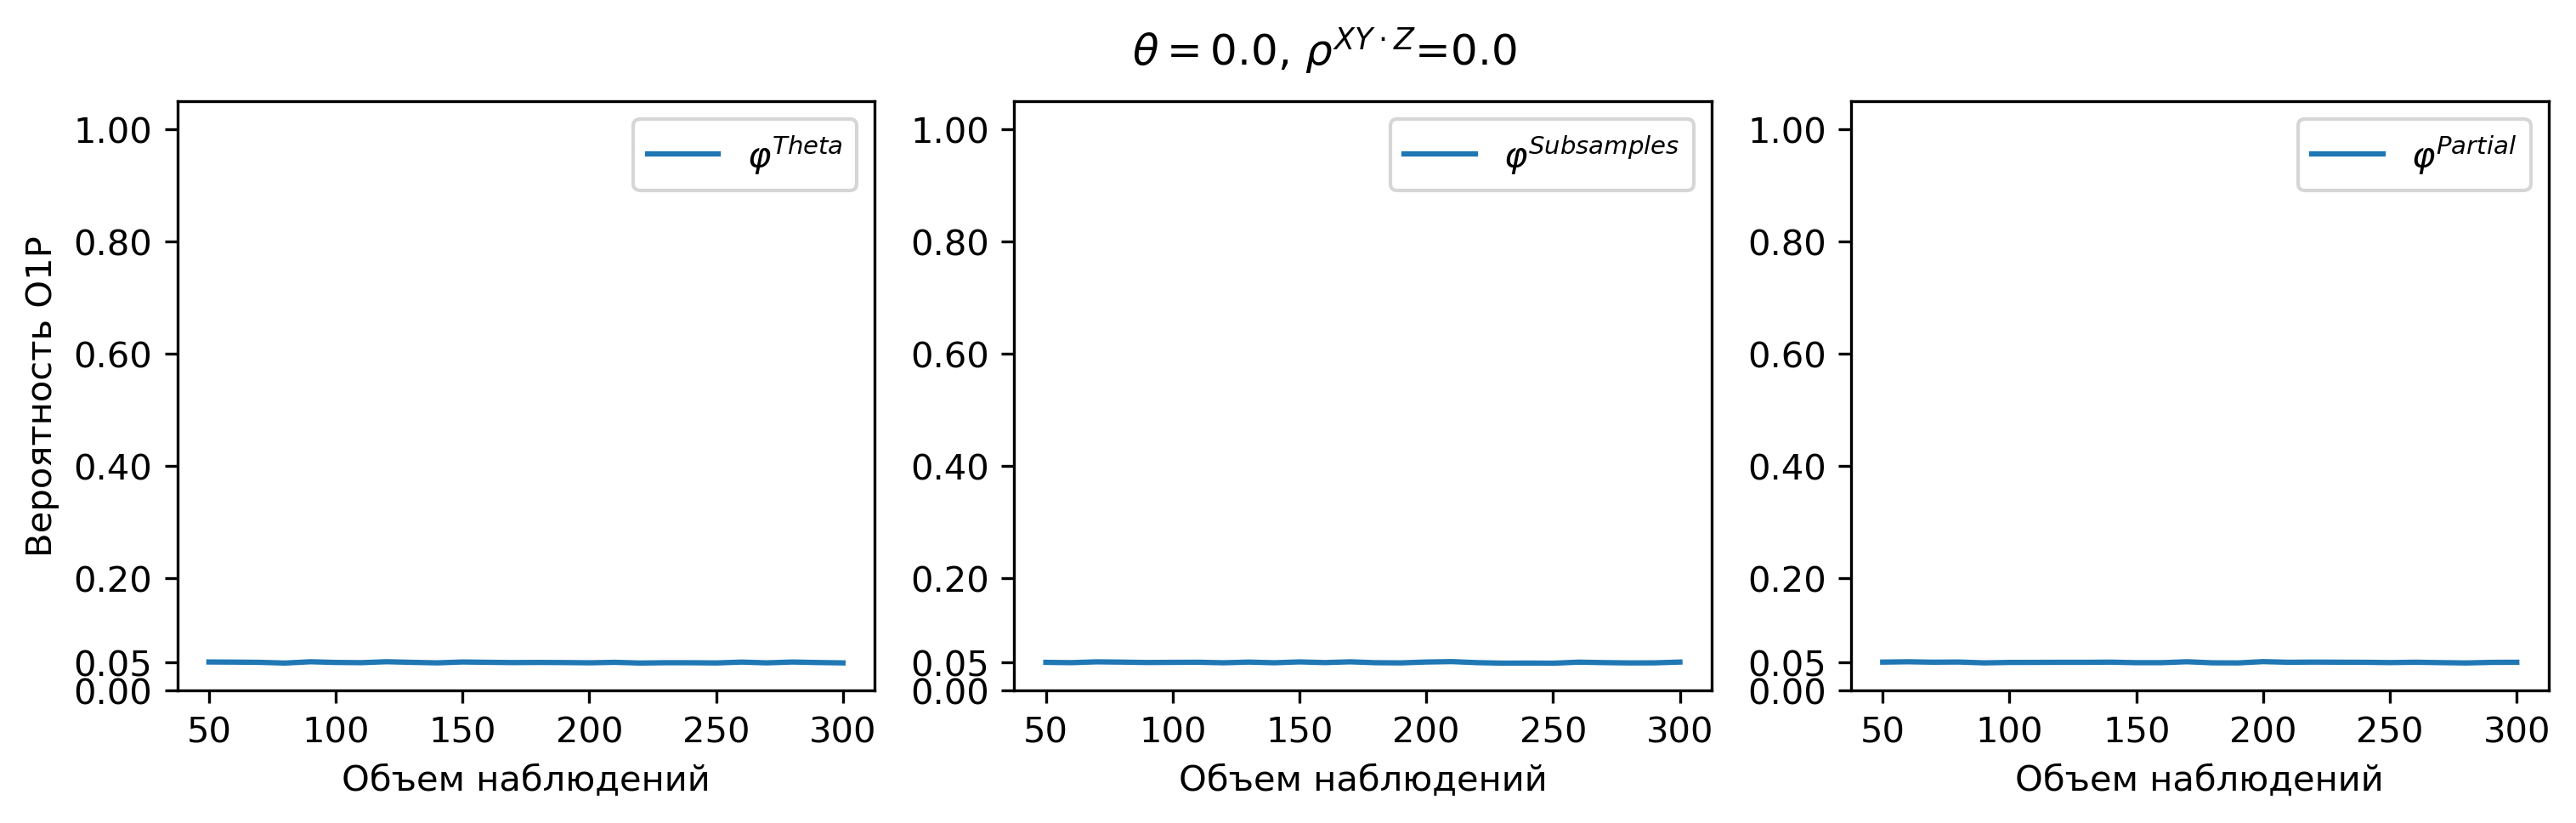
\includegraphics[scale=0.5]{images/graph1.png}
    \caption{Графики зависимости вероятности ошибки 1 рода (О1Р) от количества наблюдений,
     $p_{000}=0.125, p_{001}=0.125, p_{010}=0.125, p_{011}=0.125,
    p_{100}=0.125, p_{101}=0.125, p_{110}=0.125, p_{111}=0.125$. 
    Гипотеза $H: X \ci Y \mid Z$ верна.
    Вероятность оценивается по $10^5$ экспериментам.} \label{fig:1}
\end{figure}
    

\begin{figure}[H]
    \centering
    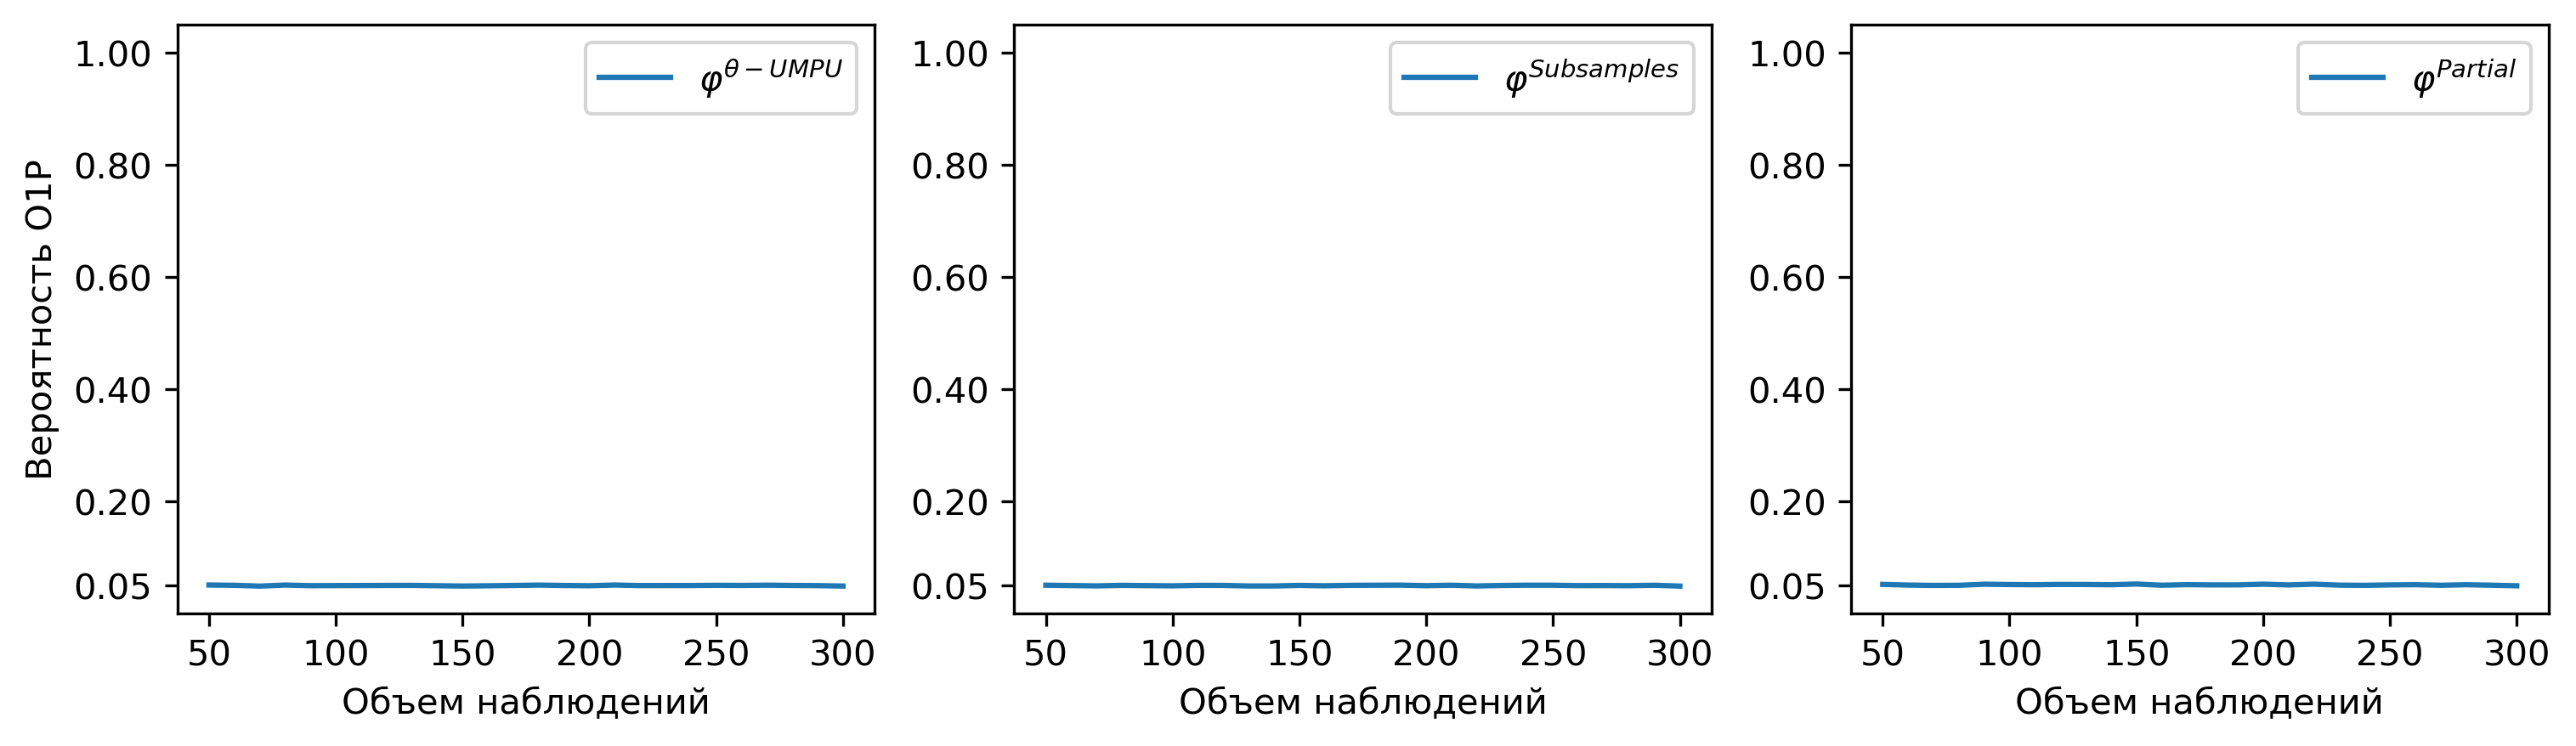
\includegraphics[scale=0.5]{images/graph2.png}
    \caption{Графики зависимости вероятности ошибки 1 рода (О1Р) от количества наблюдений,
    $p_{000}=0.15, p_{001}=0.1, p_{010}=0.3, p_{011}=0.1,
    p_{100}=0.05, p_{101}=0.1, p_{110}=0.1, p_{111}=0.1$. 
    Гипотеза $H: X \ci Y \mid Z$ верна.
    Вероятность оценивается по $10^5$ экспериментам.} \label{fig:2}
\end{figure}

\begin{figure}[H]
    \centering
    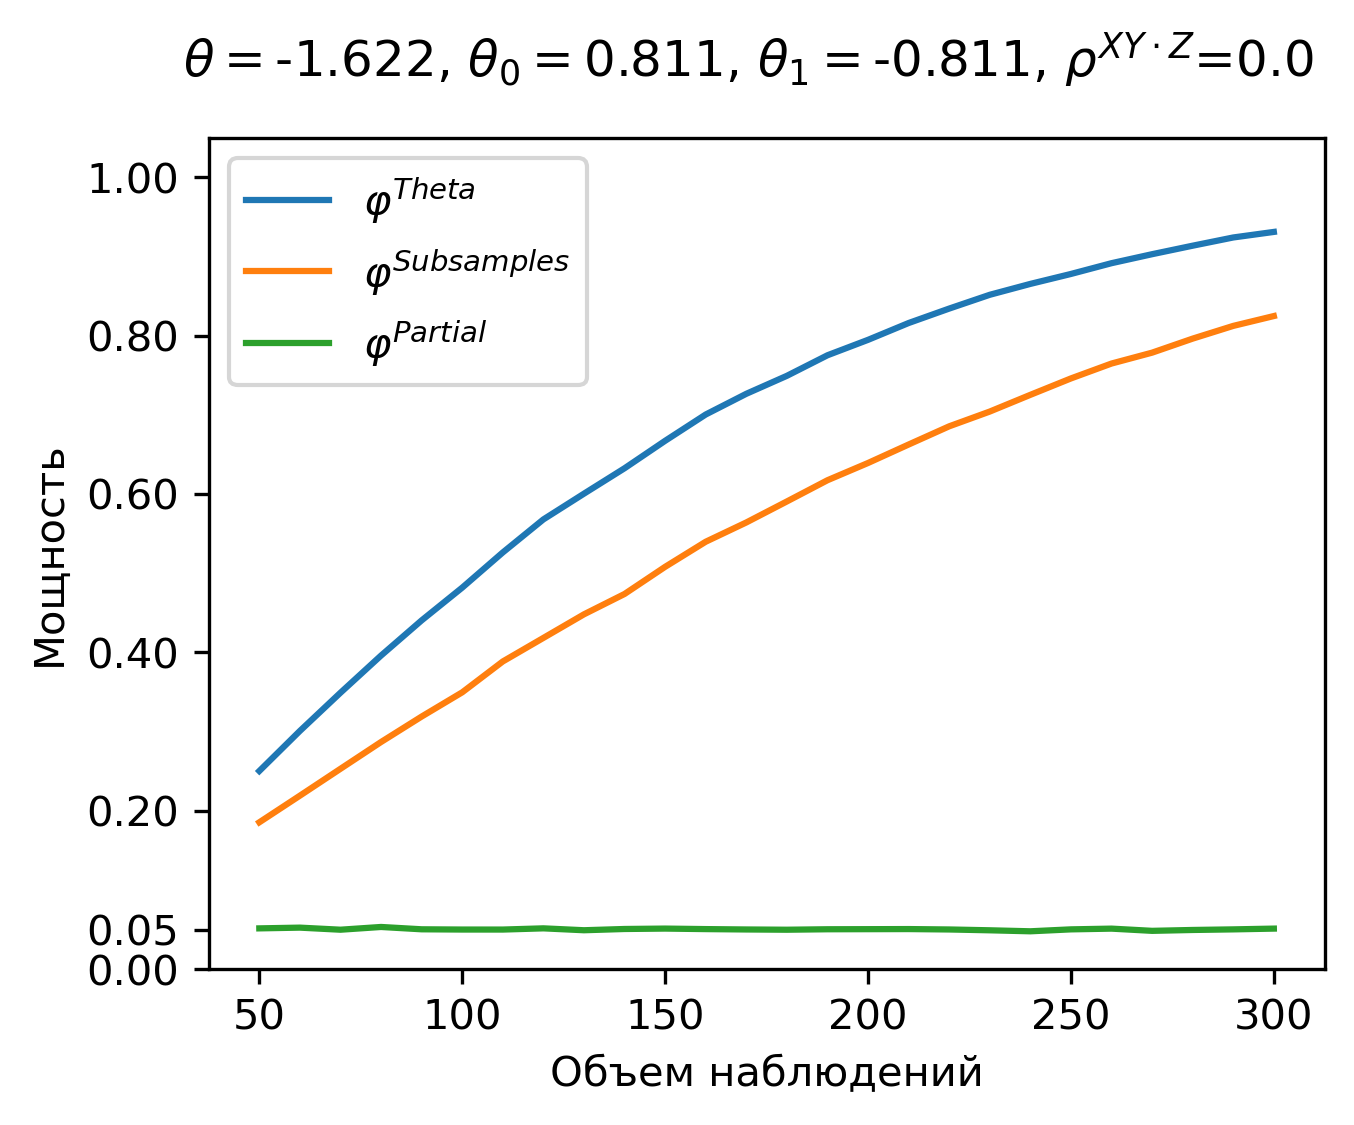
\includegraphics[scale=0.55]{images/graph4.png}
    \caption{График зависимости мощности от количества наблюдений,
    $p_{000}=0.15, p_{001}=0.1, 
    p_{010}=0.1, p_{011}=0.15,
    p_{100}=0.1, p_{101}=0.15, p_{110}=0.15, p_{111}=0.1$. 
    Гипотеза $H: X \ci Y \mid Z$ не верна, 
    однако верна гипотеза 
    $H^{\text{Partial}}: \rho^{XY\cdot Z}=0$.
    Мощность оценивается по $10^5$ экспериментам.} \label{fig:4}
\end{figure}

Из (\autoref{fig:1}) и (\autoref{fig:2}) видно, что 
для гипотезы $H: X \ci Y \mid Z$ тесты 
$\varphi^{\text{Theta}}$, $\varphi^{\text{Subsamples}}$, контролируют вероятность 
ошибки первого рода на уровне $\alpha=0.05$. Этот результат
полностью согласуется с теорией из \autoref{expon_form_section}, 
\autoref{twos}.

(\autoref{fig:1}), (\autoref{fig:2}), (\autoref{fig:4}) показывают,
что тест $\varphi^{\text{Partial}}$ контролирует вероятность
ошибки первого рода на уровне $\alpha=0.05$ для гипотезы
$H^\text{Partial}: \rho^{XY\cdot Z}=0$ в трехмерном
распределении Бернулли. Этот результат является неожиданным,
поскольку тест $\varphi^{\text{Partial}}$ теоретически обоснован
лишь для трехмерного нормального распределения.
Поскольку из $X \ci Y \mid Z$
следует $\rho^{XY\cdot Z}=0$, то тест $\varphi^{\text{Partial}}$ также
контролирует вероятность ошибки первого рода на уровне $\alpha=0.05$
и для гипотезы $H: X \ci Y \mid Z$, что показано на 
(\autoref{fig:1}), (\autoref{fig:2}).
Однако, стоит отметить,
что $\varphi^{\text{Partial}}$ проверяет необходимое условие 
условной независимости. Поэтому может возникнуть ситуация
как на (\autoref{fig:4}), когда гипотеза $H: X \ci Y \mid Z$ не верна, 
но тест $\varphi^{\text{Partial}}$ не распознает отклонение от условной независимости, поскольку
контролирует вероятность ошибки первого рода 
на уровне $\alpha=0.05$ для гипотезы $H^{\text{Partial}}: \rho^{XY\cdot Z}=0$.

\begin{figure}[H]
    \centering
    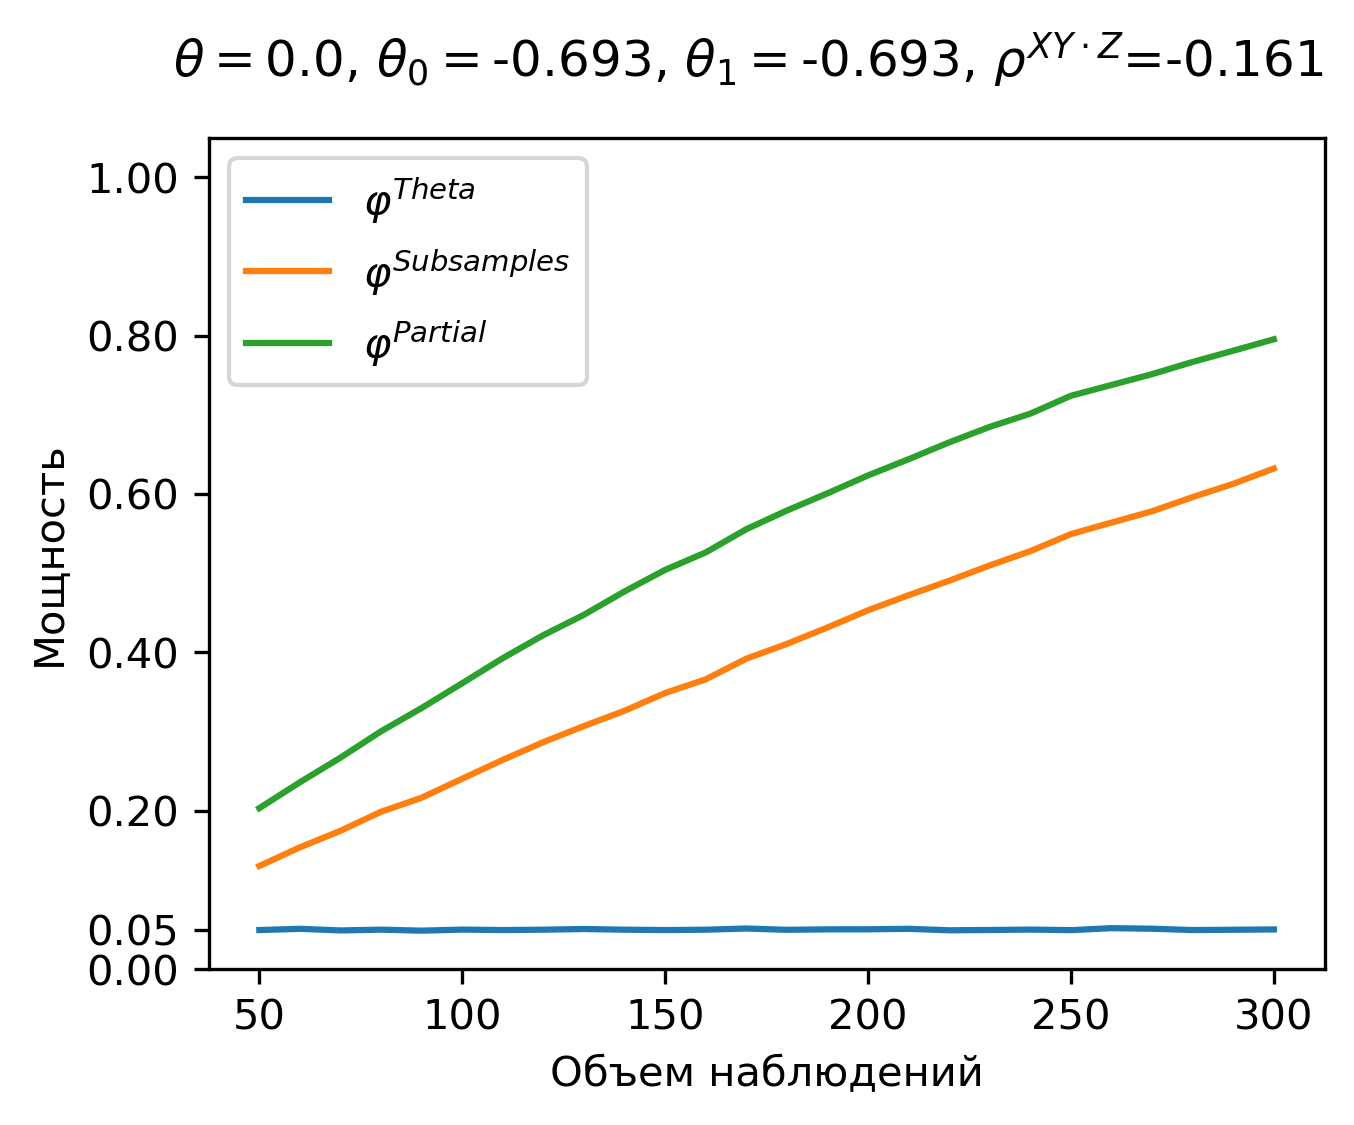
\includegraphics[scale=0.55]{images/graph5.png}
    \caption{График зависимости мощности от количества наблюдений,
    $p_{000}=0.15, p_{001}=0.05, 
    p_{010}=0.3, p_{011}=0.1,
    p_{100}=0.1, p_{101}=0.1, p_{110}=0.1, p_{111}=0.1$. 
    Гипотеза $H: X \ci Y \mid Z$ не верна, однако верны гипотезы $H^{\text{Theta}}: \theta=0$
    и $H^{\prime}: Y \ci Z \mid X$.
    Мощность оценивается по $10^5$ экспериментам.} \label{fig:5}
\end{figure}

Напомним, что тест 
$\varphi^{\text{Theta}}$ проверяет необходимое условие условной
независимости. Так на (\autoref{fig:5}) гипотеза 
$H: X \ci Y \mid Z$ не верна, 
но тест $\varphi^{\text{Theta}}$
не распознает отклонение от условной независимости и контролирует вероятность ошибки первого рода
на уровне $\alpha=0.05$ для гипотезы $H^{\text{Theta}}: \theta=0$.

Отметим, что $\varphi^{\text{Theta}}$ -- несмещенный тест уровня
$\alpha$ проверки гипотезы $H: X \ci Y \mid Z$.
Так как по \autoref{unbias} тест $\varphi^{\text{Subsamples}}$
является несмещенным тестом уровня $\alpha$ проверки гипотезы $H: X \ci Y \mid Z$, и 
на (\autoref{fig:5})
тест $\varphi^{\text{Subsamples}}$ мощнее теста $\varphi^{\text{Theta}}$,
то тест $\varphi^{\text{Theta}}$ не является РНМН тестом проверки 
гипотезы $H: X \ci Y \mid Z$, хотя является РНМН тестом
проверки гипотезы $H^{\text{Theta}}: \theta=0$.

\begin{figure}[H]
    \centering
    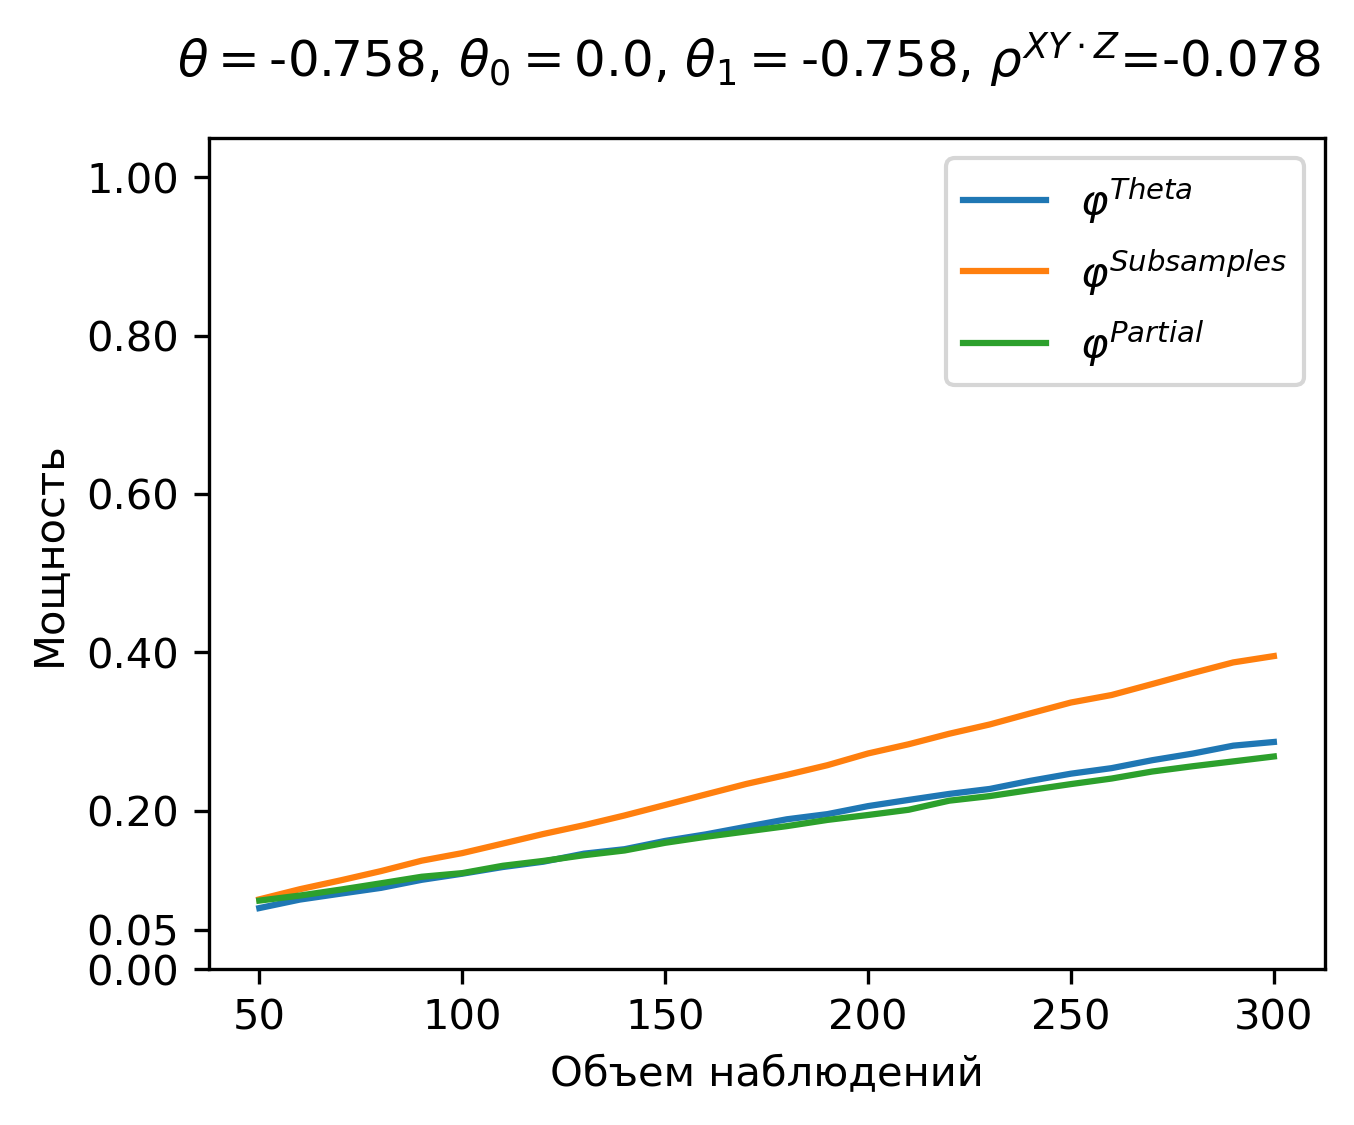
\includegraphics[scale=0.55]{images/graph3.png}
    \caption{График зависимости мощности от количества наблюдений,
    $p_{000}=0.15, p_{001}=0.06, 
    p_{010}=0.3, p_{011}=0.16,
    p_{100}=0.05, p_{101}=0.08, p_{110}=0.1, p_{111}=0.1$. 
    Гипотеза $H: X \ci Y \mid Z$ не верна, однако $X$ и $Y$ независимы
    при условии $Z=0$. 
    Мощность оценивается по $10^5$ экспериментам.}\label{fig:3}
\end{figure}

\begin{figure}[H]
    \centering
    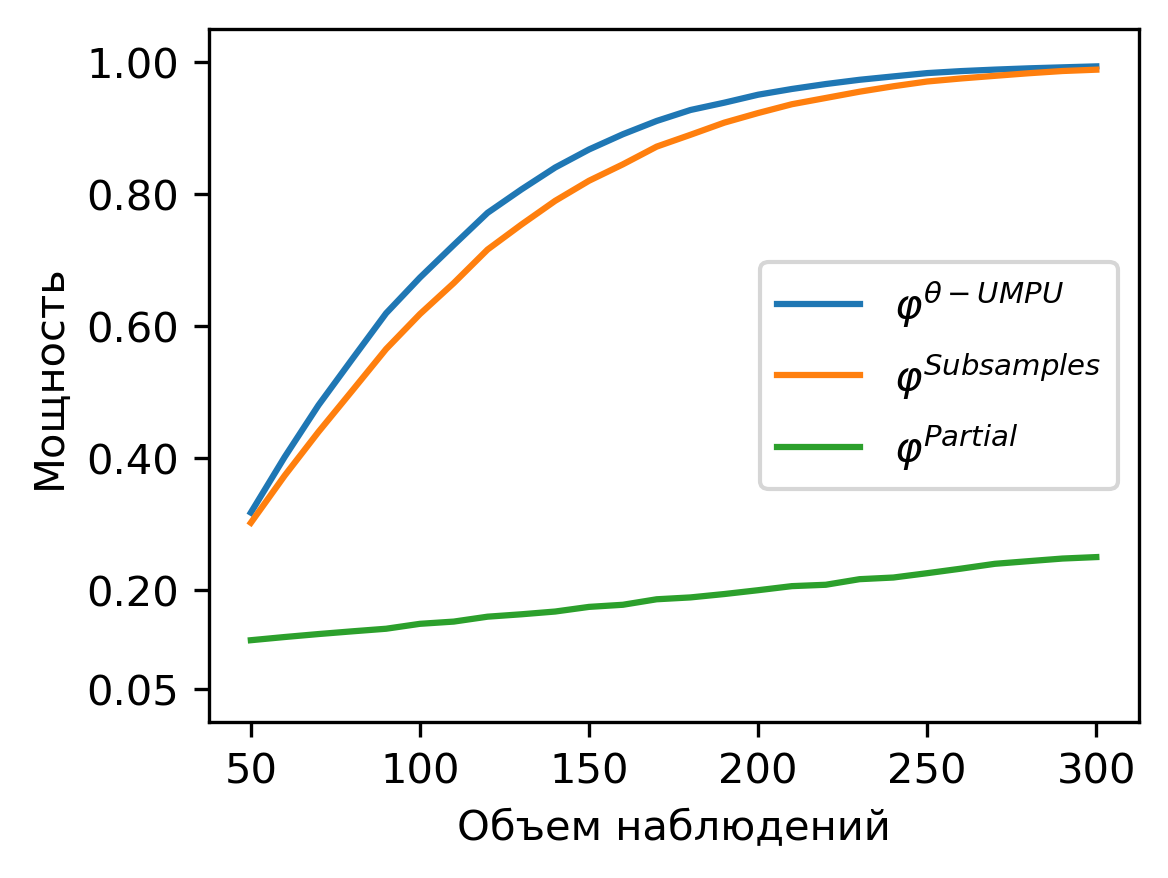
\includegraphics[scale=0.55]{images/graph6.png}
    \caption{График зависимости мощности от количества наблюдений,
    $p_{000}=0.03, p_{001}=0.1, 
    p_{010}=0.04, p_{011}=0.08,
    p_{100}=0.3, p_{101}=0.1, p_{110}=0.07, p_{111}=0.28$. 
    Гипотеза $H: X \ci Y \mid Z$ не верна.
    Мощность оценивается по $10^5$ экспериментам.} \label{fig:6}
\end{figure}

\begin{figure}[H]
    \centering
    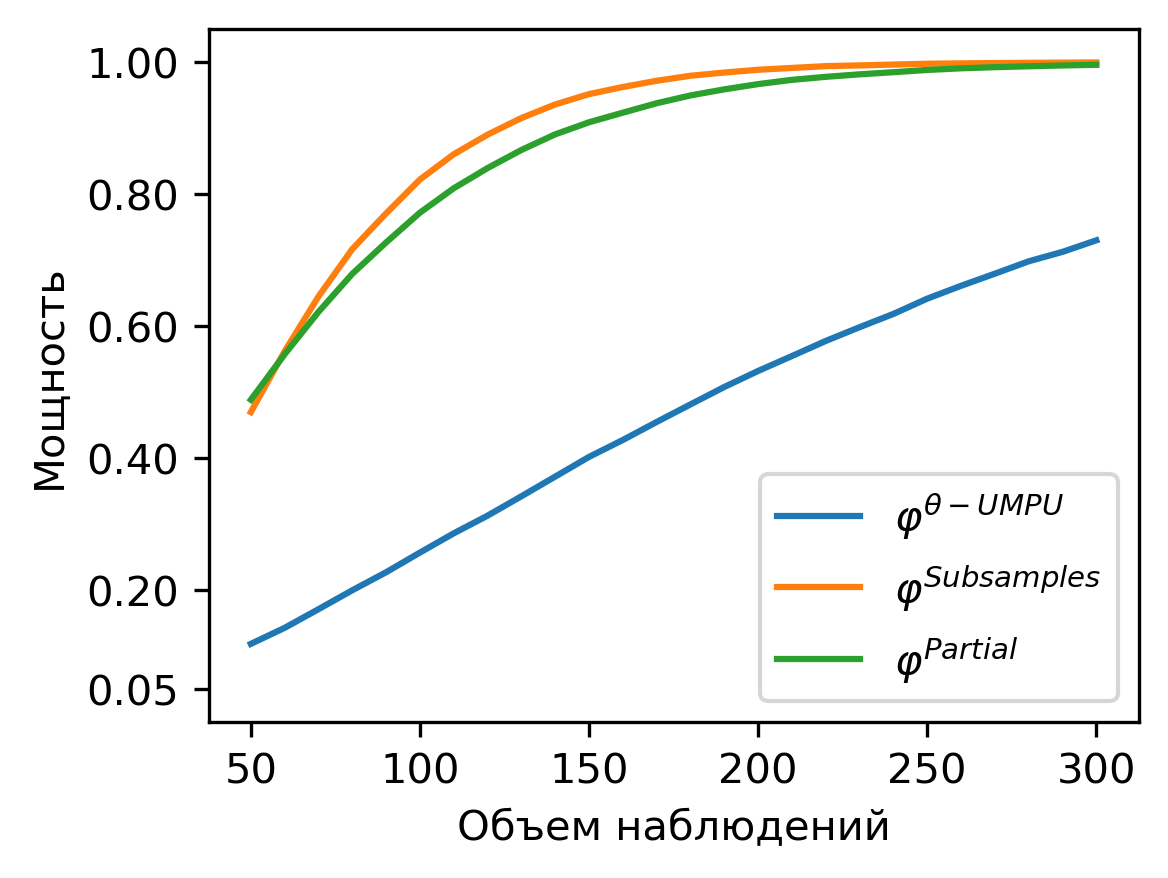
\includegraphics[scale=0.55]{images/graph7.png}
    \caption{График зависимости мощности от количества наблюдений,
    $p_{000}=0.21, p_{001}=0.12, 
    p_{010}=0.04, p_{011}=0.34,
    p_{100}=0.1, p_{101}=0.12, p_{110}=0.02, p_{111}=0.05$. 
    Гипотеза $H: X \ci Y \mid Z$ не верна.
    Мощность оценивается по $10^5$ экспериментам.} \label{fig:7}
\end{figure}

(\autoref{fig:4}), (\autoref{fig:5}), 
(\autoref{fig:3}), (\autoref{fig:6}), (\autoref{fig:7})
показывают, что, вообще говоря, рассматриваемые тесты нельзя упорядочить по мощности.
Кроме того, несмещенные тесты $\varphi^{\text{Subsamples}}$
и $\varphi^{\text{Theta}}$ уровня $\alpha$ проверки
гипотезы $H: X \ci Y \mid Z$ также нельзя упорядочить по мощности.
Поэтому вопрос построения РНМН теста проверки гипотезы 
$H: X \ci Y \mid Z$ остается открытым. 


% Одним из возможных отклонений от условной независимости является случай,
% когда $X$ и $Y$ независимы при условии $Z=0$, но зависимы при условии $Z=1$.
% Пример (\autoref{fig:3}) показывает, ...

% Показательным является пример с (\autoref{fig:6}). Тесты 
% $\varphi^{\text{Theta}}$ и $\varphi^{\text{Subsamples}}$ при $n=300$
% наблюдениях имеют мощность, близкую к $1$. В то время как мощность
% теста $\varphi^{\text{Partial}}$ приблизительно равна $0.25$. Это происходит потому, что
% в данном примере значение $\rho^{XY\cdot Z}=0.068$ близко к нулю.


% Еще интересен пример с (\autoref{fig:7}). 
% При $n=300$ наблюдениях мощность тестов
% $\varphi^{\text{Subsamples}}$, $\varphi^{\text{Partial}}$ близка к $1$,
% в то время как мощность теста $\varphi^{\text{Theta}}$ примерно равна $0.73$.

% В данном разделе были изложены результаты численных экспериментов с тестами
% $\varphi^{\text{Theta}}$, $\varphi^{\text{Subsamples}}$, 
% $\varphi^{\text{Partial}}$ при $\alpha=0.05$. На 
% (\autoref{fig:1}) и (\autoref{fig:2}) показано, что 
% при истинности гипотезы  
% $h: X \ci Y \mid Z$ эти тесты контролируют вероятность ошибки первого рода
% на уровне $\alpha=0.05$. 
% Однако, за счет того, что тесты 
% $\varphi^{\text{Subsamples}}$ и
% $\varphi^{\text{Partial}}$ проверяют более широкие гипотезы,
% возникают ситуации как на 
%  (\autoref{fig:4}) и (\autoref{fig:5}), когда гипотеза $h: X \ci Y \mid Z$
% не верна и мощность теста равна $0.05$ при любом объеме наблюдений.
% Особым образом можно выделить тест $\varphi^{\text{Subsamples}}$.
% На всех графиках $\varphi^{\text{Subsamples}}$ либо лучший по мощности,
% либо незначительно уступает лучшему по мощности тесту.


\newpage
\section*{Заключение}
\addcontentsline{toc}{section}{Заключение}
В настоящей выпускной квалификационной работе 
были получены следующие результаты:
\begin{enumerate}
    \item Сформулирован и доказан критерий условной независимости
    в трехмерном распределении Бернулли.
    \item Доказано, что ненулевое значение
    частного коэффициента корреляции Пирсона 
    $\rho^{XY \cdot Z}$ является достаточным
    условием условной зависимости $X$ и $Y$ при 
    условии $Z$ в трехмерном распределении Бернулли.
    Однако, нулевое значение $\rho^{XY \cdot Z}$ не позволяет сделать выводы
    об условной независимости или зависимости.
    \item Эмпирически, при объеме наблюдений $50 \leq n \leq 300$,
    показано, что тест
    $\varphi^{\text{Partial}}$ является тестом уровня
    $\alpha$ проверки гипотезы $H^{\text{Partial}}: \rho^{XY\cdot Z}=0$ 
    против альтернативы $K^{\text{Partial}}: \rho^{XY\cdot Z}\neq 0$
    в трехмерном распределении
    Бернулли.
    \item В экспоненциальной форме записи трехмерного 
    распределения Бернулли найден параметр 
    $\theta = \ln  \left(\dfrac{p_{001}p_{111}p_{010}p_{100}}{p_{011}p_{101}p_{000}p_{110}}\right)$,
    ненулевое значение которого является достаточным 
    условием условной зависимости всех пар
    случайных величин.
    При нулевом значении параметра $\theta$ требуются дополнительные
    исследования условных зависимостей в случайном векторе.
    \item Построен РНМН-тест $\varphi^{\text{Theta}}$
    уровня $\alpha$ проверки гипотезы $H^{\text{Theta}}: \theta~=~0$
    против альтернативы $K^{\text{Theta}}: \theta\neq 0$.
    \item Построен тест $\varphi^{\text{Subsamples}}$ 
    уровня $\alpha$
    проверки гипотезы $H: X \ci Y \mid Z$.
\end{enumerate}


% % библиография
\newpage
% \nocite{*}
\addcontentsline{toc}{section}{Список литературы}
\printbibliography
\end{document}
